%
% PRINCIPIO DE DOCUMENTO
%
\documentclass[11pt,a4paper,twoside]{book} %
\usepackage[english]{babel}

\usepackage{epsfig}
\usepackage{graphicx}
\usepackage{latexsym}

% symbols
\usepackage{amssymb,amsmath}

%Paquetes necesarios para rgb.tex
\usepackage{colordvi}
\usepackage[usenames,dvipsnames]{color}
\usepackage{fancybox}

%Paquete para pemitir multifila y multicolumnas en tablas
\usepackage{multirow}
\usepackage{multicol}

\usepackage{url}
\usepackage{listings}
\lstset{frame=single,breaklines=true,basicstyle=\footnotesize}


%para que funcione el guionado de final de linea
\usepackage[english]{babel}
\usepackage[latin1]{inputenc}
\usepackage[T1]{fontenc}


\usepackage{longtable}
\usepackage{url}

%%
% CARACTERES ESPECIALES DE USO COMUN EN CASTELLANO
% Definiciones v�lidas para latex
%
%                            Valent�n Carde�oso
%

\typeout{* Estilo spain.sty. (C) 1993 valent�n}
\def\hoy{\number\day\space{de}\space\ifcase\month\or
 Enero\or Febrero\or Marzo\or Abril\or Mayo\or Junio\or
 Julio\or Agosto\or Septiembre\or Octubre\or Noviembre\or Diciembre\fi
 \space{de}\space\number\year}

% RELATIVO A LOS CARACTERES PROPIOS DEL IDIOMA
\catcode`�=\active
\catcode`�=\active
\catcode`�=\active
\catcode`�=\active
\catcode`�=\active
\catcode`�=\active
\catcode`�=\active
\catcode`�=\active
\catcode`�=\active
\catcode`�=\active
\catcode`�=\active
\catcode`�=\active
\catcode`�=\active
\catcode`�=\active
\catcode`�=\active
\catcode`�=\active
\catcode`�=\active
\catcode`�=\active
\catcode`�=\active
\catcode`�=\active

\gdef�{\'{a}}
\gdef�{\'{e}}
\gdef�{\'{\i}}
\gdef�{\'{o}}
\gdef�{\'{u}}
\gdef�{\~{n}}
\gdef�{\'{A}}
\gdef�{\'{E}}
\gdef�{\'{I}}
\gdef�{\'{O}}
\gdef�{\'{U}}
\gdef�{\"{u}}
\gdef�{\"{U}}
\gdef�{\~{N}}
\gdef�{\c{c}}
\gdef�{\c{C}}
\gdef�{!`}
\gdef�{?`}
\gdef�{$\rm^o$}
\gdef�{$\rm^a$}


%para el formato del pseudoc�digo incluido en el capitulo cluster

%%%%%%%%%%%%%%%%%%%%%%%%%%%%%%%%%%%%%%%%%%%%%%%%%%%%%%%%%%%%%%%%
%
% Longitudes
%
%%%%%%%%%%%%%%%%%%%%%%%%%%%%%%%%%%%%%%%%%%%%%%%%%%%%%%%%%%%%%%%%
\newdimen\indentedTextWidth              % longitud de texto sangrado
\indentedTextWidth=\textwidth
\advance\indentedTextWidth - \parindent

\newdimen\twoIndentedTextWidth           % longitud de texto sangrado 2 veces
\twoIndentedTextWidth=\textwidth
\advance\twoIndentedTextWidth - \parindent
\advance\twoIndentedTextWidth - \parindent


\newdimen\EjBodyW                   % anchura del cuerpo de los ejemplos
\newdimen\EjBodyH                   % altura del cuerpo de los ejemplos
\newdimen\EjGap                     % espaciado del body con header y footer
\newdimen\EjTotalH                  % altura total del ejemplo
\newdimen\EjHeaderB
\newdimen\EjHeaderH
\newdimen\EjFooterB
\EjGap=1cm
%%%%%%%%%%%%%%%%%%%%%%%%%%%%%%%%%%%%%%%%%%%%%%%%%%%%%%%%%%%%%%%%
%
% Contadores
%
%%%%%%%%%%%%%%%%%%%%%%%%%%%%%%%%%%%%%%%%%%%%%%%%%%%%%%%%%%%%%%%%
\newcounter{ContEj}[chapter]
%%%%%%%%%%%%%%%%%%%%%%%%%%%%%%%%%%%%%%%%%%%%%%%%%%%%%%%%%%%%%%%%
%
% commando: \doubleLine{width}
%
%%%%%%%%%%%%%%%%%%%%%%%%%%%%%%%%%%%%%%%%%%%%%%%%%%%%%%%%%%%%%%%%
\newcommand{\doubleLine}[1]
{\makebox[0pt][l]{\rule[0.1mm]{#1}{0.4pt}\par}\rule{#1}{0.4pt}}
%%%%%%%%%%%%%%%%%%%%%%%%%%%%%%%%%%%%%%%%%%%%%%%%%%%%%%%%%%%%%%%%
%
% commando: \singleLine{width}
%
%%%%%%%%%%%%%%%%%%%%%%%%%%%%%%%%%%%%%%%%%%%%%%%%%%%%%%%%%%%%%%%%
\newcommand{\singleLine}[1]{\makebox{\rule[0pt]{#1}{0.4pt}\par}}
%%%%%%%%%%%%%%%%%%%%%%%%%%%%%%%%%%%%%%%%%%%%%%%%%%%%%%%%%%%%%%%%
%
% commando \parOval[rightText]{leftText}
%
%%%%%%%%%%%%%%%%%%%%%%%%%%%%%%%%%%%%%%%%%%%%%%%%%%%%%%%%%%%%%%%%
\newcommand*{\parOval}[2][\ ]
{
  \newpage
  {\noindent{\shadowbox{\makebox[\textwidth][s]{#2 #1}}\\\par}}
}
%%%%%%%%%%%%%%%%%%%%%%%%%%%%%%%%%%%%%%%%%%%%%%%%%%%%%%%%%%%%%%%%
%
% commando: \begin{tableXMLSchema}{caption}{label}
%                  elemento con la sintaxis
%           \hline
%                  schema XML
%           \end{tableXMLSchema}
%
%%%%%%%%%%%%%%%%%%%%%%%%%%%%%%%%%%%%%%%%%%%%%%%%%%%%%%%%%%%%%%%%
\newenvironment*{tableXMLSchema}[2]
{
  \begin{longtable}{|p{\textwidth}|}
    %
    % Caption de la Tabla
    %
      \caption{#1}
      \label{#2} \\
    %
    % S�lo aparece en el la primera p�gina de la tabla
    %
      \hline
      \\
      \endfirsthead
    %
    % Aparece al principio de las sucesivas p�ginas
    %
      \caption[]{#1} \\
      (\ldots continuaci�n) \\ \\
      \endhead
    %
    % Aparece al final de cada p�gina
    %
      \\
      (contin�a en la siguiente p�gina \ldots)\\
      \endfoot
    %
    % Aparece al final de la tabla
    %
      \hline
      \endlastfoot
    %
    % Contenido de la tabla
    %
}
{
  \end{longtable}
}
%%%%%%%%%%%%%%%%%%%%%%%%%%%%%%%%%%%%%%%%%%%%%%%%%%%%%%%%%%%%%%%%
%
% commando \refexample
%
%%%%%%%%%%%%%%%%%%%%%%%%%%%%%%%%%%%%%%%%%%%%%%%%%%%%%%%%%%%%%%%%
\newcommand*{\refexample}{\stepcounter{ContEj}Pseudoc�digo \thechapter.\theContEj\ }
%%%%%%%%%%%%%%%%%%%%%%%%%%%%%%%%%%%%%%%%%%%%%%%%%%%%%%%%%%%%%%%%
% commando \begin{example}[comentario]{Ancho}{Alto}{Label}
%          \end{example}
%
%%%%%%%%%%%%%%%%%%%%%%%%%%%%%%%%%%%%%%%%%%%%%%%%%%%%%%%%%%%%%%%%
\newsavebox{\captionEj}
\newsavebox{\Ej}
\newsavebox{\comentarioEj}
\newenvironment*{example}[4][\ ]
{
  \EjBodyW=#2
  \EjBodyH=#3
  \label{#4}
  \sbox{\captionEj}{\textcolor{Black}{\small{\textbf{\refexample}}}}
  \sbox{\comentarioEj}{#1}
  \begin{lrbox}{\Ej}
    \begin{minipage}[t]{#2}
}
{
    \end{minipage}
  \end{lrbox}
  \EjTotalH=\EjBodyH
  \advance\EjTotalH \EjGap
  \EjHeaderB=0.5\EjTotalH
  \advance\EjHeaderB -0.25cm
  \EjFooterB=-0.5\EjTotalH
  \advance\EjFooterB -0.25cm
  \EjHeaderH=0.5\EjTotalH
  \advance\EjHeaderH -0.15cm \noindent
  \rule[-0.5\EjTotalH]{0.1pt}{\EjTotalH}
  \makebox[-3pt][l]{\hspace{-3pt}\rule[-0.5\EjTotalH]{0.5cm}{0.1pt}}\rule[0.5\EjTotalH]{0.5cm}{0.1pt}
  \makebox[0pt][l]{\hspace{-3pt}\rule[\EjHeaderB]{0.1pt}{0.5cm}}
  \makebox[0pt][l]{\hspace{-7pt}\rule[\EjFooterB]{0.1pt}{0.5cm}}
\makebox[0pt][l]{\raisebox{\EjHeaderH}{\colorbox{White}{\usebox{\captionEj-}}{\usebox
\comentarioEj}}}
  \makebox[0pt][l]{\hspace{-20pt}\raisebox{0.375\EjBodyH}{\usebox{\Ej}}}
%  \makebox[0pt][l]{ \hspace{-15pt}\raisebox{-0.5\EjTotalH}{\usebox{\comentarioEj}}}
\\
\\
}


%%%%%%%%%%%%%%%%%%%%%%%%%%%%%%%%%%%%%%%%%%%%%%%%%%%%%%%%%%%%%%%%
% commando \begin{attributeList}{width}{headerText}
%          \end{attributeList}
%
%%%%%%%%%%%%%%%%%%%%%%%%%%%%%%%%%%%%%%%%%%%%%%%%%%%%%%%%%%%%%%%%
\newenvironment*{attributeList}[2]
{
  \vspace{0.5cm}
  \parskip=0pt
\par\noindent{\makebox[0pt][l]{\rule[1mm]{\textwidth}{0.4pt}\par}\rule{\textwidth}{0.4pt}}
\par
  \textsc{atributos} de #2\par
  \noindent\rule[0pt]{\textwidth}{0.4pt}
  \noindent
  \begin{list}{}{ \labelwidth=#1
                  \setlength{\leftmargin}{\labelwidth}
                  \addtolength{\leftmargin}{\labelsep}}
  \vspace{-0.5cm}
}
{
  \end{list}
\vspace{-\parsep}
\noindent{\makebox[0pt][l]{\rule[1mm]{\textwidth}{0.4pt}\par}\rule{\textwidth}{0.4pt}}
\par \vspace{0.5cm}
}


%fichero con el guionado al final de linea
% Para que funcione la divisi�n por guiones es necesario incluir los paquetes:
% \usepackage[T1]{fontenc}
% \usepackage[spanish]{babel}
% \usepackage[latin1]{inputenc}

% Vocabulario en INGL�S
\hyphenation{ BPMI car-trid-ges cre-a-ting ma-nu-fac-tu-ring MDA
Mo-del Mo-de-ler re-a-li-za-tion re-sul-ting spe-cia-li-zed
a-dap-ta a-dap-ta-ci�n a-dap-tan a-dap-t�n-do-se a-dap-tar
a-dap-tar-se a-dap-tas ad-mi-nis-trar ad-mi-nis-tra-ci�n
ad-mi-nis-tra-cio-nes ad-mi-nis-tran-do ad-mi-nis-tra-ti-va
ad-mi-nis-tra-ti-vas ad-mi-nis-tra-ti-vo ad-mi-nis-tra-ti-vos
a-n�-li-sis a-na-li-za-da a-na-li-za-das a-na-li-za-do
a-na-li-za-dos a-na-li-zan-do a-na-li-zan-do-se a-na-li-zar
a-na-li-za-r�an an-te-rior an-te-rior-men-te an-te-rio-res
a-pro-pia-da a-pro-pia-das a-pro-pia-do a-pro-pia-dos
a-pro-ve-cha-da a-pro-ve-cha-das a-pro-ve-cha-do a-pro-ve-cha-dos
a-pro-ve-chan-do a-pro-ve-char a-proxi-ma-ci�n
ar-qui-tec-t�-ni-cos au-to-des-cri-bir-se au-to-ma-ti-ca
au-to-ma-ti-cas au-to-ma-ti-co au-to-ma-ti-cos au-to-ma-ti-za-ci�n
au-to-ma-ti-za-da au-to-ma-ti-za-das au-to-ma-ti-za-do
au-to-ma-ti-za-dos au-to-ma-ti-zar au-to-ri-za-da au-to-ri-za-das
au-to-ri-za-do au-to-ri-za-dos be-ne-fi-cia be-ne-fi-cia-da
be-ne-fi-cia-das be-ne-fi-cia-do be-ne-fi-cia-dos be-ne-fi-cian
be-ne-fi-ci�n-do-se be-ne-fi-ciar be-ne-fi-ciar-se be-ne-fi-cias
be-ne-fi-cia-se be-ne-fi-cia-sen be-ne-fi-cio be-ne-fi-cios bien
ca-rac-te-r�s-ti-ca ca-rac-te-r�s-ti-cas ca-rac-te-r�s-ti-co
ca-rac-te-r�s-ti-cos cen-trar-nos cen-trar-se co-la-bo-ra-ci�n
co-la-bo-ra-cio-nes co-la-bo-ra-dor co-la-bo-ra-do-ra
co-la-bo-ra-do-ras co-la-bo-ra-do-res co-la-bo-ran-do co-la-bo-rar
con-cre-ta con-cre-ta-men-te con-cre-tar con-cre-tas con-cre-to
con-cre-tos con-fi-gu-ra-ci�n con-fi-gu-ra-cio-nes con-fi-gu-ra-da
con-fi-gu-ra-das con-fi-gu-ra-do con-fi-gu-ra-dos con-fi-gu-ran-do
con-fi-gu-rar con-si-de-ra con-si-de-ra-ci�n con-si-de-ra-cio-nes
con-si-de-ra-da con-si-de-ra-das con-si-de-ra-do con-si-de-ra-dos
con-si-de-ra-mos con-si-de-ran-do con-si-de-r�n-do-la
con-si-de-r�n-do-las con-si-de-r�n-do-lo con-si-de-r�n-do-los
con-si-de-r�n-do-se con-si-de-rar con-si-de-re con-si-de-r�
con-si-de-re-mos con-si-de-ren con-si-d�-ren-se con-si-de-res
cons-truc-ci�n cons-truc-cio-nes cons-tru-ir cons-tru-ir-la
cons-tru-ir-las cons-tru-ir-lo cons-tru-ir-los cons-tru-yen
cons-tru-yen-do cons-tru-y� con-ti-nua con-ti-nua-ci�n
co-rres-pon-da co-rres-pon-dan co-rres-pon-de co-rres-pon-den
co-rres-pon-den-cia co-rres-pon-den-cias co-rres-pon-des
co-rres-pon-dien-do co-rres-pon-dien-do-se co-rres-pon-dien-te
co-rres-pon-dien-tes cre-a-ci�n cre-a-cio-nes cre-ar
de-fi-ni-ti-va de-fi-ni-ti-vas de-fi-ni-ti-vo de-fi-ni-ti-vos
de-no-mi-na-ci�n de-no-mi-na-da de-no-mi-na-das de-no-mi-na-do
de-no-mi-na-dor de-no-mi-na-do-res de-no-mi-na-dos de-no-mi-nan
de-no-mi-nar de-pen-dien-do de-pen-dien-te de-pen-dien-tes
de-sa-rro-lla de-sa-rro-lla-do de-sa-rro-lla-dor
de-sa-rro-lla-do-res de-sa-rro-lla-dos de-sa-rro-llan-do
de-sa-rro-llo de-sa-rro-llos des-cri-be des-cri-ben des-cri-bes
des-cri-bir des-cri-bi-r� des-cri-bi-r�n des-cri-bien-do
des-cri-bien-do-les des-crip-ci�n des-crip-cio-nes des-cri-ta
des-cri-tas des-cri-to des-cri-tos des-pu�s de-ta-lla de-ta-lla-da
de-ta-lla-das de-ta-lla-do de-ta-lla-dos de-ta-llan-do de-ta-llar
de-ta-llas de-ta-lle de-ta-lles di-fe-ren-cia di-fe-ren-cian-do
di-fe-ren-ciar di-fe-ren-cias di-fe-ren-te di-fe-ren-tes di-se-�a
di-se-�a-dor di-se-�a-do-ra di-se-�a-do-res di-se-�ar di-se-�as
di-se-�o di-se-�os dis-po-ni-bi-li-dad dis-po-ni-ble
dis-po-ni-bles do-cu-men-to do-cu-men-tos e-jem-plar e-jem-pla-res
e-jem-plo e-jem-plos e-le-men-to e-le-men-tos e-li-mi-na
e-li-mi-n�is e-li-mi-nan e-li-mi-nan-do e-li-mi-nan-do-lo
e-li-mi-nar e-li-mi-nas e-li-mi-nes e-li-mi-no e-li-mi-n�
em-pre-sa-rial em-pre-sa-ria-les en-ru-ta-mien-to es-ce-na-rio
es-ce-na-rios es-ce-ni-fi-car e-sa e-sas e-so e-sos
es-pe-ci-fi-ca-ci�n es-que-ma-ti-za-do e-va-l�-a e-va-lua-ci�n
e-va-lua-cio-nes e-va-l�-an e-va-l�-an-do e-va-lu-ar e-va-l�-as
e-xac-ta e-xac-ta-men-te e-xac-tas e-xac-ti-tud e-xac-to e-xac-tos
e-xis-te e-xis-ten e-xis-ten-cia fa-ci-li-tan fa-ci-li-tan-do
fa-ci-li-tar flexi-bi-li-dad flexi-bi-li-zar ge-ne-ra ge-ne-ra-da
ge-ne-ra-das ge-ne-ra-do ge-ne-ra-dos ge-ne-ral ge-ne-ra-les
ge-ne-ra-li-za-ci�n ge-ne-ras ge-ne-ro ge-ne-ros ges-ti�n
ges-tio-nar ges-tio-na-ble ges-tio-na-bles ges-tio-nes ges-tor
ges-to-res ha-bi-tu-al-men-te he-rra-mien-ta he-rra-mien-tas}







%tama�os
\textwidth=12cm %14
\textheight=19cm
\parskip=1.5ex
\topmargin=1.5cm
%he modificado los valores para los margenes de impresion a doble cara
\oddsidemargin=2.5cm  %1.5
\evensidemargin=1.42cm  %.46

%distancia del encabezado al texto
\headsep=1.2cm


%para modificar el estilo de los encabezados de p�gina

%hay q ponerlo siempre despu�s de pagestyle headings
\pagestyle{headings}
\renewcommand*{\chaptermark}[1]{\markboth{\small\upshape\scshape\thechapter.
\ #1}{}}
\renewcommand*{\sectionmark}[1]{\markright{\small\upshape\scshape\thesection.
\ #1} }


% P�ginas blancas sin cabecera
%  para p�ginas izquierdas que s�lo incluyen cabeceras

\makeatletter
\renewcommand*{\cleardoublepage}
{ \clearpage \if@twoside
  \ifodd\c@page
\else
  \hbox{}
  \thispagestyle{empty}
  \newpage
  \if@twocolumn
    \hbox{}
    \newpage
  \fi
\fi \fi } \makeatother




\begin{document}



\setcounter{secnumdepth}{5}

\pagestyle{empty}
%%%%%%%%%%%%%%%%%%%%%%%%%%%%%%%%%%%%%%%%%%%%%%%%%%%%%%%%%%%%%%%%%%%%%%%%%%%%%
%%%%%%%%%%%%%%%%%%%%%%%%%%%%%%%%%%%%%%%%%%%%%%%%%%%%%%%%%%%%%%%%%%%%%%%%%%%%%
%
% PORTADA
%
%%%%%%%%%%%%%%%%%%%%%%%%%%%%%%%%%%%%%%%%%%%%%%%%%%%%%%%%%%%%%%%%%%%%%%%%%%%%%
%%%%%%%%%%%%%%%%%%%%%%%%%%%%%%%%%%%%%%%%%%%%%%%%%%%%%%%%%%%%%%%%%%%%%%%%%%%%%
\begin{center}
\ \\
\vskip -2cm \epsfxsize=4cm \epsffile{escudousal}
\\
\
\\
{\LARGE{\sc Universidad de Salamanca}}\\
\vskip 5mm

{\Large{Departamento de Inform�tica y Autom�tica}}\\



\vskip 2.7cm
{\huge \bf{ \scshape Semantic}}\\
\vskip 0.2cm
{\huge \bf{ \scshape RESTful}}\\
\vskip 0.2cm
{\huge \bf{ \scshape Web}}\\
\vskip 0.2cm
{\huge \bf{ \scshape Services}}\\
\vskip 1cm {\large \sc Master's Thesis} \vskip 1cm
{\large \sc Templated created by Dra. D�a. Montserrat Mateos S�nchez}\\
\vskip 3cm
{\large \bf Directed by:}\\
\vskip 0.2cm
{\large {\sc Template reviewed b Dr. D. Jos� Luis Alonso Berrocal}}\\
\vskip 0.1cm \vskip 1cm {\large Julio 2006}

\end{center}

\newpage \pagestyle{empty} \mbox{}
\newpage

\setcounter{page}{1}
%%%%%%%%%%%%%%%%%%%%%%%%%%%%%%%%%%%%%%%%%%%%%%%%%%%%%%%%%%%%%%%%%%%%%%%%%%%%%
%%%%%%%%%%%%%%%%%%%%%%%%%%%%%%%%%%%%%%%%%%%%%%%%%%%%%%%%%%%%%%%%%%%%%%%%%%%%%
%
% PORTADA
%
%%%%%%%%%%%%%%%%%%%%%%%%%%%%%%%%%%%%%%%%%%%%%%%%%%%%%%%%%%%%%%%%%%%%%%%%%%%%%
%%%%%%%%%%%%%%%%%%%%%%%%%%%%%%%%%%%%%%%%%%%%%%%%%%%%%%%%%%%%%%%%%%%%%%%%%%%%%
\begin{center}
\ \\
\vspace{-3cm} \epsfxsize=4cm \epsffile{escudousal}
\\
\
\\
\textbf{\Large UNIVERSIDAD DE SALAMANCA}\\
%\\
\vspace{2mm}
{\Large \bf{Departamento de Inform�tica y Autom�tica}}\\
\vspace{3cm}
{\huge \bf{ \scshape Semantic}}\\
\vspace{0.2cm}
{\huge \bf{ \scshape RESTful}}\\
\vspace{0.2cm}
{\huge \bf{ \scshape Web}}\\
\vspace{0.2cm}
{\huge \bf{ \scshape Services}}\\

\vskip 2cm {\large \sc Master's Thesis authored by:}\\
\vskip 0.2cm {\large \sc D.Antonio Garrote Hern'andez} \vskip 1cm
{\large \bf Dirigida por:}\\
\vskip 0.2cm
{\large {\sc Dr. Da. Mar'ia Moreno Montero}}\\
\vskip 1cm \noindent\begin{tabular}{p{3cm}p{1cm}p{3cm}p{1cm}p{3cm}}
\centerline{Master en Sistemas Inteligentes} \\
\end{tabular}
\vskip 2cm \rightline{\large Salamanca,September 2009}
\end{center}

\newpage \pagestyle{empty}\mbox{}
\newpage

\

\



\noindent {\Large Pepe P�rez, {\it Profesor Catedr�tico de Escuela
Universitaria del Departamento de Inform�tica y Autom�tica de la
Universidad de Salamanca}

 \

\noindent {\bf HACE CONSTAR}: {\it Que} D. Jos� P�rez P�rez, {\it
Ingeniero Inform�tico por la Universidad de Salamanca ha realizado
bajo mi direcci�n la Memoria que lleva por t�tulo} T�tulo de la
tesis realizada, {\it con el fin de obtener el grado de Doctor por
la Universidad de Salamanca}.

\

\noindent Y para que surta los efectos oportunos firmo en Salamanca,
a veintisiete de Julio de dos mil seis.

}

\newpage \pagestyle{empty}\mbox{}
\newpage
\pagestyle{plain}
\chapter*{Agradecimientos}

No quer�a dejar pasar esta oportunidad para recordar y agradecer a
todas aquellas personas que .....

.....


Gracias.

\chapter*{Resumen}

La Web constituye un enorme espacio de informaci�n digital
distribuida, en el que los usuarios tienen a su disposici�n
vol�menes ingentes de informaci�n ....

\chapter*{Abstract}
The Web provides a large space of digital distributed information in
which the users can find huge amounts of dynamic and heterogeneous
information. To be able to search for and retrieve pertinent and
interesting information the user....


%\newpage
%\pagestyle{empty} \mbox{}
%\newpage

%\newpage
%\pagestyle{empty} \mbox{}
%\newpage
%\chapter*{Agradecimientos}

No quer�a dejar pasar esta oportunidad para recordar y agradecer a
todas aquellas personas que .....

.....


Gracias.



%para cambiar el formato de la numeraci�n de p�ginas a romano
%\setcounter{page}{1}
%\renewcommand{\thepage}{\roman{page}}

%para que en las tablas aparezca "tabla" y no "cuadro"
\renewcommand\listtablename{�ndice de tablas}
\renewcommand{\tablename}{{\bf Tabla}:} \pagestyle{plain}

\tableofcontents

\listoftables

\listoffigures
%\newpage
%\pagestyle{empty} \mbox{}
%\newpage
%\setcounter{page}{1}

\pagestyle{headings}
\renewcommand*{\chaptermark}[1]{\markboth{\small\upshape\scshape\thechapter.
\ #1}{}}
\renewcommand*{\sectionmark}[1]{\markright{\small\upshape\scshape\thesection.
\ #1} }

%para cambiar el formato de la numeraci�n de p�ginas a ar�bigo
%\renewcommand{\thepage}{\arabic{page}}

\chapter{Introduction}

World Wide Web Consortium (W3C) director's Tim Berners Lee, introduced the term Semantic Web in a seminal article in 2001\cite{berners-lee_semantic_2001} to designate his long term vision of what
the web should become. This vision involved the creation of a meta data layer on top of the existent web data describing the
meaning, the semantics, of these data. These semantic meta data would be necessary to enable automatic reasoning by software
web agents, that will retrieve and combine these data, inferring new facts when required, in order to fulfill the needs of the users
they work for. In the words of Berners Lee "The Semantic Web will bring structure to the meaningful content of Web
pages, creating an environment where software agents roaming from page to page can readily carry out sophisticated tasks
for users".\\

In the eight years that have passed since its original conception, a big effort to materialize this disruptive vision of
the web has been carried out. Organizations like the W3C, academic institutions and to a lesser degree, commercial
companies, have built foundational technologies that could enable the kind of applications envisioned by Berners Lee. 
Despite all these efforts, the Semantic Web remains today an ambitious idea yet to become true. The adoption of semantic
technologies by main stream web sites is small, semantic web applications are scarce and not well known, and even the
tools required for building semantic applications are not in a mature stage of development. This lack of success
combined with the initial high expectations set about what the Semantic Web could achieve has led to many people to consider
the Semantic Web just another buzzword that will never have an actual realization.\\

This state of things has originated the opinion that if the Semantic Web is to become a reality, it would be required a more
pragmatic solution to the problem of bridging the gap between today's web and the future Semantic Web. Before disruptive
semantic applications involving automatic reasoning can be a
reality, it is necessary that web applications start supporting semantic technologies situated at the base of the
semantic web technologies stack.  This will only be possible if the
entry barrier for the adoption of semantic technology is low and its benefits for the users or developers of a web
application real and immediate. Semantic technologies like annotated RDF (RDFa) that describes an easy mechanism for
inserting semantic meta data into HTML documents, that have met almost instant support by search engines, are steps into this direction. \\

This work tries to be a small contribution to this effort, describing a way for web developers and architects to design
and build their applications in terms of semantic web services that follows the core design principles of the HTTP
protocol. This will allow them to build, in a highly productive way, open systems with standard semantic meta data as
their main building blocks.

\section{The Semantic Web initiative and its promises}

The semantic web initiative was from its very conception a description of the web as a set of data resources that could be processed
in an automatic way by software applications. Under this conception, the main mechanism used by
software agents when processing data in the semantic web would be logical inference. The goal of enabling automatic
reasoning by software agents in the web has defined the main steps and technologies being developed under the semantic web
initiative. The outcome of this initiative has specified a set of layers on top of the HTTP protocol and the HTML mark up language, the core web
technologies, that make up a system for symbolic reasoning in the web. These layers include a formal syntax for facts provided
by XML, RDF and RDFS, an ontology description layer provided by OWL with roots in the description logics field and
current work in rules languages that can be used in conjunction with OWL like SWRL.\\

Using all these technologies it could be possible to develop web agents capables of achieving tasks that could only be
acomplished through the inference of new facts from data previously retrieved from the web. Classical examples of those tasks
are automatic biding and purchasing of goods, arrangement of appointments or the recommendation and filtering
of contents based on its semantic description.\\

Under this concdeption of the Semantic Web, additional layers are required for the building of semantic web applications and
agents. These layers involve dealing with the problem of uncertainty \cite{uncertaintyweb}. The proof and trust layers in the semantic web stack should provide mechanisms to enable
safe inference of new facts to web agents. Current research in this field include adopting theorical developments in
probability theory, fuzzy logic and belief functions.\\

At the top of semantic web initiative road map is the user interface and applications layer. This layer should provide
the mechanisms for a user to make actual use of the semantic web capabilities provided by the underlying semantic
technologies and standards.

\section{Current issues preventing the adoption of semantic technologies}

The Semantic Web initiative, as many attempts of drive radical technological change, is suffering from a bootstrap
problem. Current semantic technologies require widespread adoption to provide real benefits for their users, but users do not adopt
those technologies because they cannot be easily applied to present day web problems. \\

As we have mentioned, Semantic Web's development ultimate goal has been the achievement of automatic reasoning by software
agents in the web.  This vision of the web is in many ways radically different from today's web and so are the challenges
semantic web technologies like OWL and SPARQL try to solve. The problem most of these technologies face is that
while semantic web technological stack remains unfinished, adoption of these technologies has to come from nowadays
application developers. An important barrier preventing the adoption of semantic technologies by today's web developers is the relatively
complexity of these technologies. Technologies like OWL or rule systems require for their use the understanding of a
complex theoretical background that contrasts sharply with the simplicity of  main stream web technologies. \\

Another serious problem discouraging semantic web technologies adoption is the focus semantic technologies on symbolic
reasoning. Semantic standards provide the means to store facts in web documents that can be used in automatic inference,
but today's web is already fulfilled with unstructured data that cannot be easily annotated with semantic meta data. If these data are to
be used as a subject of knowledge for the Semantic Web they need to be processed in an automatic way, using statistical
techniques to produce annotated meta data with a certain degree of certainty. Another important concern is how to trust
facts exposed by semantic web data repositories. It is required that Semantic Web
technologies can cope with the concepts of uncertainty and probability, enabling the data mining of semantic data. \\

There is also a misunderstanding of use cases for semantic technologies. In absence of semantic web applications with
big user bases, there are no examples of how semantic technologies can be used to deliver more useful solutions. It is
necessary to find ways of applying semantic technologies to current issues in web development so they can serve as
example of semantic technology applicability capable of boosting further adoption.


\section{Lowercase Semantic Web}

As a reaction to the current situation of the semantic web, there has been a recent raise of interest in the use of
semantic web technologies to achieve improvements in problems found in current web application's design and
implementation. This kind of developments have been sometimes referred to as "lowercase semantic web''. This field was pioneered
by projects like the microformats project \url{http://microformats.org}, that tries to provide an easy way for
inserting semantics into HTML documents. They distinguished themselves by a stronger focus in delivering actual
improvements for web users, applying semantic technologies in pragmatic ways in today's web applications.\\

Search engines for instance, have started to parse semantic formats in web pages, as well as microformats, trying to obtain more accurate search
results for their users. Application developers are using microformats as a lightweight and easy to understand
alternatives to ontology languages like OWL, focusing in data exchange rather than automatic inference. \\

This pragmatic approach to the Semantic Web constitutes a bottom-up attempt of materializing the Semantic Web, building on
top of present day technologies, and trying to solve current problems, like the open exchange of data, with semantic standards.

\section{Opportunities for the semantic web}

Despite all these impediments, the current state of the web offers many chances to boost the adoption of semantic web
technologies. Current tendencies in the way of building web applications suppose an increase in the importance of data in the web.  Web
design is evolving at a fast pace from n-tier architectures where data persistence and business logic  were executed in the server and then rendered as HTML documents in the web browser, to a
model where business logic and rich user interfaces are executed in the browser and only persistence of data is provided
by the server. We are moving from a web of application servers and browsers to a web of web services and rich clients.
The following are some examples of this change in the way of developing web applications:

\begin{itemize}
\item The interest in Javascript execution engines by browser developers like Mozilla,
Apple or Google. 
\item The raise of rich Javascript frameworks based on the model view controller architecture like Sproutcore or
  Capuccino
\item The release of rich internet application development platforms like Adobe Flex, Java FX or Microsoft Silverligth.
\item The interest in key value stores as an alternative to relational data bases
\end{itemize}


Services must be carefully designed to expose data in an efficient way. Furthermore, today's web applications are built on top of data
from multiple providers, services like Google Maps or Twitter, are mashed up with other data to provide innovative
functionalities to the users. Besides, web agents are not anymore restricted to web browsers, a new generation of mobile
devices connected to the internet are consuming web data in mobile devices conforming what has been described as the
diffuse web \cite{conf/coordination/Serrano09}.\\

As important as the access to web data from web clients is the need of exchanging data from different providers. To
offer actual value to web users, interoperability for web data must be achieved, but the current situation shows data
providers using ad hoc data schemas and web services.\\

Semantic web technologies can be used to provide an easy and flexible solution to the problem of the generation, and
exchange of open data in the web. Semantic technologies can be also used in conjunction with new data persistence tools to
provide a powerful alternative to traditional relational data base driven web applications.\\

If easy ways of inserting web technologies in nowadays web development stacks are provided to web developers, it could
boost the adoption of web technologies and constitute the foundation for more advanced layers of semantic technology. 


\section{Goals of this work}

In this document we describe how pragmatic use of web technologies in current web applications can be
achieved through the use of what we have named RESTful semantic web services.\\

The plan of this document starts with the description of a very simple formal model that can be used to describe semantic web data
providers and consumers. Then, a specification of this model is built using standard semantic web technologies. This
specification is transformed later into an actual implementation of a client and server software libraries that can be
used to build semantic web applications with RESTful semantic web services. Finally, we describe one of
the applications that can be built with the described software libraries. It can serve as a sample of the kind of
applications that can be built with the technologies introduced.\\

Our main ambition is to propose feasible technological solutions for current day web development problems, for instance,
the open exchange of data between web services and rich internet clients. This solution uses semantic web technologies as a mean for solving these problems
but as a side effect, it conforms a basic layer where the whole semantic web stack of technologies could be delivered later. This technological
solution must be built on top of a valid theoretical base, useful for the description and design of web architectures, and must
adhere itself to the simplicity of the REST principles. Focusing on simplicity and productivity, without rejecting the use of standard semantic technologies, we try to provide
an attractive platform for developers that could help to boost the growth of the Semantic Web.
\chapter{Formal Description of RESTful Semantic Web Services  \label{capituloFD}}

\section{Introduction}
In this chapter I will describe a formal language that allows the description of computational model based on the consumption
and composition of semantic RESTful web services.\\

The aim of this formulation is to provide a solid foundation for the development of a technical specification and
posterior implementation of mechanisms to expose, exchange and consume semantic meta data through semantic web services
and REST principles. The availability of a formal framework for the description of services is also a crucial step for
addressing a number of important questions involving automatic reasoning about services and semantic meta data, like
service composition or bi-simulation.\\

This basis of this formal language draws heavily from the theory of
Pi-Calculus \cite{Milner99communicating} and other process calculi and from classic work on Tuple Space Computing
\cite{Gelernter85generativecommunication}.\\

Using this formal language a system can be described consisting of a group of HTTP agents, exposing resources as
triple spaces. The state of these triples spaces can be modified according to REST semantics, by exchanging HTTP messages between agents
participating in a distributed computation. The communication channel between agents are HTTP connections to the URIs
inserted into the services triples meta data. From this point of view, the agents are mobile agents, since the
communication channels that allows the reception of incoming messages can move from agent's triple space to agent's
triple space through several HTTP messages. In the model, the communication channels are typed. This fact imposes
restrictions on the triples that can be inserted or removed from the agents' triple spaces. The specification of this
restrictions on the communications channels will be exposed as services descriptions.

\section{State of the Art}
The formal specification of web services have been a field of great activity in recent years. The commercial interest in
Service Oriented Architectures (SOA) of web services has originated a great number of works from academic and practitioners, around the formal
specification of web services work flows, trying to solve the problems of web services orchestration and web services
choreography.  All these efforts have crystallized into the creation of standard languages for
the description of web services work flows like the Web Services Business Process Execution Language (WS-BPEL)
\cite{Fu04analysisof},  or the Web Services Choreography Description Language (WS-CDL)
\cite{Burdett:05:WSC}. These standardization efforts have been influenced by principles of Pi-Calculus like the passing
of channels between participants \cite{chan08chor}. \\

These description languages participate in a conception of SOA computing based in the use of heavy weight web services
(WS-*). This means that the same problems appearing in other WS-* specifications are also present in these services, one
major problem being the complexity of the specifications. This complexity prevents the formal specification of these
languages using some kind of calculus. Nevertheless, there have been attempts of building complete process calculi for
these standards as in \cite{Lucchi05api-calculus} or \cite{Lapadula07acalculus}. \\

In the field of semantic web services, the adoption of semantic standards with its foundation in description logics,
provides an optimal basis for the formal description of web services. Some standards likeprovide similar features for the formal description of semantic web services. These standards proposals
mix the power of description logics to describe the service meta data with some kind of logic language (SWRL, KIF, DRS,
ROWS, FLOWS),  to describe preconditions and postconditions regulating the orchestration and choreography of web
services. Other semantic web services proposals like Web Services Semantics (WSDL-S)  \cite{wsdls}  propose the reuse of
existent standards like BPEL extending them with semantic annotations.\\

All these semantic web services proposals build their models around the syntax of WS-* web services, extending their
technologies (SOAP, WSDL, UDDI) with a semantic layer. This very conception of web services have received recently much
criticism because of its perceived lack of congruence with the web architecture they use as a transportation layer. This
ciricism has centered in the meaningless use of URIs, the great coupling between clients and services, and the rejection
of the state-less archtecture of the web \cite{FieldingTaylor02toit}. The concerning about the breaking of the principles of the web, as
they were exposed in the specification of the HTTP protocol has resulted in alternative proposals for web services
construction,  founded on the seminal work on Representational State Transfer (REST) \cite{Fiel00} architectures
proposed by Thomas Fielding. \\

These news ideas about web services architectures have had also its influence in the field of semantic web services
specifications. Resemblances between RESTful architectures and Tuple Spaces architectures for parallel computation have
been drawn \cite{Fensel04triple-spacecomputing:} in proposals for Triple Spaces computing, where the resources metadata are
exposed as sets of triples. Under both paradigms, the information is published by agents into a persisten memory space  and then consumed asynchronally
by other agents. In the the tuple space paradigm the information has the form of sets of tuples, collections of ordered
fields, meanwhile the web information consists of web resources like HTML pages. In both models expose an uniform and minimal interface to access this spaces and the agents communicating
through the information stored in the memory spaces does not need to know each other. In this proposal, shortcomings about the lack of structure in the tuple spaces \cite{journals/jss/JohansonF04} are solved by
the use of the RDF triple graph model \cite{Hayes:04:RS} to encode the resources model representation in triple spaces. The agents
accesing these triples spaces would use the classical tuple space operations to manipulate the triples stored in these
triple spaces. Som extensions to these primitive operations have been proposed for a most convinient interface to the
stored triples \cite{Simperl07acoordination}.

\section{Mixing triple spaces and pi calculus}
As it has been shown in the previous section, triple spaces provides a promising foundation for the construction of
semantic web services that are congruent with the REST principles of the web. 
Nevertheless, we think that triple space computing, as it has been formulated, is not enough to provide a full formal
model for semantic web services. For instance, it does not provide a way of describing formally how an agent must access different
triple spaces in order to fullfill some kind of computation or the interaction between different agents through the
publishing and consumption of triple from triple spaces. These problems have been a long time concern in the world of WS-* web services under the term of orchestration and
choreography of web services.\\
Besides, it can be argued that some aspects of the triple space proposal clash with main features of RESTful architectures, as the differences between the
operations over triple spaces and HTTP verbs.\\

We try to adress this issues by the formulation of a version of the Polyadic Pi-Calculus
extended to incorporate the concept of triple spaces in the process of the calculus.  
In our version of the calculus the simplest construct is a process. Each of these processes as in the original
Pi-Calculus perfom some kind of computation involving the reception and emission of messages through links acting as communication channels. The main
difference between our processes and original ones is that each process has one attached triple space. They can also
have handles granting the process access to other triple spaces may be shared between different processes.\\ These
triple spaces handle are private for each process or group or processes and cannot be exchanged between processes in
messages. If a process wishes to read the contents of the triple space attached to a remote process, it must send a
request message through a link leading to that process. As in the original Pi-Calculus for mobile processes, links
between processes, opposite to triple space handles, can be exchanged in messages between processes. Thus, in our model
we replace direct manipulation of remote triple spaces by the proxing of this manipulations to remote process through
the exchange of messages through links. Furthermore, the
triples stored in the triple space of a process can contain any number of links to new processes, and the triples
exchanged in the messages can provide acces to new process through encoded links.\\
When a process receives a message containing new triples or a request asking for the triples in its associated triple
spaces, the process may try to read or write into the triple spaces for whom he has handles. If these handles are shared
between different processes they can used the classical blocking variants of the read and write operations for tuple
spaces as a coordination mechanism between processes.\\

This description of the elements of a Pi-Calculus make up a fairly generic distributed computational model but
provides the building blocks to describe a semantic RESTful web services architecture. This can be achieved adding some
restrictions to the previous model. \\

The first of these restrictions is the need of adapting the communication mechanism between processes to the HTTP
protocol that lies at the heart of RESTful architectures. In order to accomplish this, the communication channels must
consist of HTTP connections identified by URIs. Since HTTP connections provides a bidirectional communication mechanism,
each time a message is sent through a HTTP connection to a certain URI, an anonymous link back to the process doing the
request is also sent and can be used to send a response message back. URIs, as the links in the original Pi-Calculus can
are persistent and can be exchanged between processes meanwhile the anonymous response links are efimerous and cannot be
exchanged. Since the URIs can be encoded in the triples exchanged in the calculus messages, they can also be stored in
the triple spaces associated to each process. Another important feature of our version of the calculus is that processes
can create new URIs to be used in the computation in the same way that the orignal processes in the Pi-Calculus could
introduce new names for links between processes. Another REST related feature of our version of the calculus is that
there are different kinds of messages, coincident with the verbs of the HTTP protocol, restricted in our case to the set
GET, POST, PUT and  DELETE.\\

The second restriction we need to impose deals with the support for the semantic features of the web service description
formalism. This need requires to add support for metadata describing the information exchanged by processes. In our
version of the calculus we have expressed this metadata support by the means of transforming our initial simple
Pi-Calculus into a polyadic Pi-Calculus \cite{Milner91thepolyadic}, where types can be associated to the URIs used for communication between
processes. It is also necessary to associate a type to different sets of triples, so only triples of a certain type can
be sent or read through URIs with that associated type. Besides we add templates that match the triples of a certain
type and that can be exchanged in messages and the ability to transforma certain template with an associated type into a
set of triples with an associated type through the inserton of an URI into the template.\\

With theses restrictions added to our initial models, we can describe any RESTful architecture in a formal way, by a set
of processes whose execution shows the following semantics:
\begin{itemize}
\item A semantic RESTful web service process will be modeled after a process with an unique URI of a certain type. This service will
  have stored into its private triple space the semantic representation of the service, identified by the URI of the
  service. The service process will process the incoming messages marked with the HTTP verbs, according to the semantics of the HTTP
  protocol.
\item A client will be a process without an associated public URI that will accomplish a computation sending requests to
  different service processes and modifying the contents of its associated triple space with the triples retrieved from
  these service processes.
\item A GET request will be interpreted by the remote service process as an attemp to retrieve the full set of triples
  stored into its associated triple space of a certain tpe.
\item A POST operation containing a template of a certain type will be interpreted as a request for creating a new
  nested service process, identified by a new nested URI, with an associated triple space containing the result of
  inserting the new URI in the received triple template. The new triple space will be shared between parent and child
  process.
\item A PUT operation containing a set of triples of certain type will be interpreted by the remote service process as a
  request to replace the contents of its associated triple space with the contents of the triples contained in the
  reuqest.
\item A DELETE operation to a certain URI will be interpreted by the remote service process as an attempt to emptying
  the associated triple space and finishing the execution of the process. 
\item Since a parent service process retains handles to all the triple spaces of the created processes, a GET operation
  to the parent process will return the whole content of the child triple spaces, providing a way for returning a
  listing of the processes.
\item Two client process can carry a distributed computation publishing triples into remote service process that other
  clients could retrieve later, or by the use of the tuple space operation in a shared private triple space
\end{itemize}

\section{Syntax}
In this version of the Pi-calculus the core concepts used, as in any other process calculus \cite{Tutorial91thepolyadic} \cite{Milner89acalculus}, are names, processes and channels. These concepts are extended with the concept of triple spaces: common repositories of triples associated with each process. Processes can write, read or delete triples from triple spaces. Furthermore, clients processes can share triple spaces using triple space operations as a sort of communication mechanism. Communication between clients and servers will be accomplished by the exchange of messages modelled after the HTTP protocol verbs, including values or patterns encoding triples. Channels, messages, values and patterns are typed and follow strict typing rules.\\
We will use the following symbols for the mentioned concepts:
\begin{itemize}
\item $P,Q,A,B...$ processes including servers and clients.
\item $v,w...$ values encoded as sets of triples.
\item $p,q...$ patterns matching values against sets of triples.
\item $u_1,u_2...$ handlers for triple spaces.
\item $l_1,l_2... $ channels for processes communication.
\item $m_1,m_2...$ messages exchanged through channels.
\item $T,[T],()$ types for channels, values and triples.
\end{itemize}

The syntax of the calculus is shown in grammar form:

\begin{eqnarray*}
  P,Q,A,B  & ::=  & \mbox{REST services / agents} \\
       & P | Q   & \mbox{Parallel composition} \\
    |     & P(u) | Q(u)   & \mbox{Parallel composition of processes with } \\
       &   & \mbox{Common access to the u triple space} \\
    |     & 0  & \mbox{Terminated process} \\
    |     & \mbox{{\bf new } c:T {\bf in } P} & \mbox{Creation of new channel of type T} \\
    |     & \overline{c}m  & \mbox{Sending of message m through channel c} \\
    |     & (m)c  & \mbox{Reception of a message through channel c} \\
    |  & !P  & \mbox{Process replication / spawning} \\
    |  & w(u)<v>  & \mbox{Writing of value v in the u triple space} \\
    |  & r(u)<p>  & \mbox{Non blocking reading of values matching pattern} \\
       &       & \mbox{p in the u triple space} \\
    |  & br(u)<p> & \mbox{Blocking reading of values matching pattern} \\
       &       & \mbox{p in the u triple space} \\
    |  & d(u)<v>  & \mbox{Deleting of value v in the u triple space} \\
    |  & <p,c>  & \mbox{Applies URI of channel c to the pattern p} \\
    |  & [v = p]  & \mbox{Pattern matching for value v and pattern p} \\
\end{eqnarray*}
\begin{eqnarray*}
  v,w:T & ::=  & \mbox{Triples encoded value of type T} \\
      &  (d_1 ... d_j,  & \mbox{ Set of data for data properties} \\
      &    & \mbox{ defined in triples encoded value of type T} \\
      &  c_k:T_k ... c_n:T_n)  & \mbox{ Set of object channels for object properties} \\
      &    & \mbox{ defined in triples encoded value of type T} \\
    | & [v]:[T]  & \mbox{ Collection of triples encoded values of type T} \\
    | & ()  & \mbox{ Empty set of triples} \\
  p,q:T & ::= & \mbox{Patterns of type T} \\
  u_1,u_2 .. u_n & ::= & \mbox{Triplet space handlers} \\
 m:T & ::= & \mbox{HTTP messages} \\
      & [GET,p:T_o,c:T_i]:T_o& \mbox{HTTP GET request with pattern p}\\
      &                        &\mbox{and response channel c} \\
    | & [POST,p:T_o,c:T_i]:T_o& \mbox{HTTP POST request with pattern of} \\
      &                        &\mbox{value T and response channel c} \\
    | & [PUT,v:T_o,c:T_i]:T_o & \mbox{HTTP PUT request with triplets of value} \\
      &                       & \mbox{T and response channel c} \\
   | & [DELETE,(),c:T_i]:() & \mbox{HTTP DELETE request and response channel c} \\
    | & [n,v:T_o]:T_o & \mbox{HTTP response with code n and value T}
\end{eqnarray*}

\section{Informal Semantics}

In this section we will describe informally the semantics of the calculus, discussing structural congruence, reduction rules, typing and labelled transitions.

\subsection{Structural congruence}
Free names in process X will be designated by fn(X), and bounded names by bn(X).

\begin{itemize}
\item 0: $fn(0) = bn(0) = 0 $
\item P(u):
  \begin{itemize}
    \item $fn = fn(P) - \{ u \}$
    \item $bn = \{u\} \cup bn(P)$
  \end{itemize}
\item P!:
  \begin{itemize}
    \item $fn = fn(P)$
    \item $bn = bn(P)$
  \end{itemize}
\item new x in P:
  \begin{itemize}
    \item $fn = fn(P) - \{ x \}$
    \item $bn = bn(P) \cup \{x\} $
  \end{itemize}
\item $\overline{c}m.P$:
  \begin{itemize}
    \item $fn = fn(P) \cup \{ c, m \}$
    \item $bn = bn(P) - \{ c, m\}$
  \end{itemize}
\item $(m)c.P$:
  \begin{itemize}
    \item $fn = fn(P) \cup \{ c\}$
    \item $bn = bn(P) \cup \{ m \} - \{ c\}$
  \end{itemize}
\item $(w,d)(u)<v>.P$:
  \begin{itemize}
    \item $fn = fn(P) \cup \{ v \} - \{ u \}$
    \item $bn = bn(P) \cup \{ u \} - \{ v\}$
  \end{itemize}
\item $(r,br)(u)<p>.P$:
  \begin{itemize}
    \item $fn = fn(P) \cup \{ p \} - \{ u \}$
    \item $bn = bn(P) \cup \{ u \} - \{ p\}$
  \end{itemize}
\end{itemize}
The following rules hold when checking the structural congruence ($\equiv$) of two processes.
\begin{itemize}
  \item{\bf $\alpha$ conversion}: Two processes differing exclusively in the name of bounded variables are considered congruent.
  \item{\bf $|$ is a symmetric monoid}: $P|Q\,\equiv\,Q|P,\;P|0\,\equiv\,P$
  \item $!P\,\equiv\,P|!P$
  \item $new\,x\,in\,0\,\equiv\,0,\,new\,x\,in\,(new\,y\,in\,P)\,\equiv\,new\,y\,in\,(new\,x\,in\,P)$
\end{itemize}
\subsection{Reduction}
Each process in the calculus has an associated triple space where triples can be written, read and deleted with the operators $r,br,w$ and $d$ (read, blocking read, write and delete). Additionally, processes may have access to other triple spaces $u_1,u_2 ... u_n$ expressed as $P(u_1,u_2 ... u_n)$ . In order to interpret the semantics of the calculus, we use the following structure for each process:
\begin{itemize}
  \item $TS<P> = |P|$
  \item $TS<P(u_1,u_2...u_n)> = |P| \cup |u_1| \cup |u_2| \cup ... \cup |u_n|$
\end{itemize}
Where $|P|$ is the set of triples stored in the triple space of the process $P$, $|u_i|$ is the set of triples stored in the triple space $u_i$.\\
The reduction ($\longrightarrow$) relation \cite{Sewell00appliedpi;} is the least relation which satisfies the following rules:
\begin{itemize}
  \item $COMM\,:\,TS<P>,TS<Q>\,\vdash\,(m)c.P|\overline{c}m.Q\,\longrightarrow\,TS<P>,TS<Q>\,\vdash P \bullet Q$
  \item $TSW_1\,:\,TS<P(u)>\,\vdash\,w(u)<v>.P\,\longrightarrow\, |P| \cup |u| \cup \{ v \}\,\vdash P$
  \item $TSW_2\,:\,TS<P>\,\vdash\,w<v>.P\,\longrightarrow\, |P| \cup \{ v \}\, \vdash P$
  \item $TSR_1\,:\,TS<P(u)>\,\vdash\,r(u)<p>.P\,\longrightarrow\, TS<P(u)>\,\vdash P$
  \item $TSR_2\,:\,TS<P>\,\vdash\,r<p>.P\,\longrightarrow\, TS<P>\,\vdash P$
  \item $TSD_1\,:\,TS<P(u)>\,\vdash\,d(u)<v>.P\,\longrightarrow\, |P| \cup |u| - \{v\},P$
  \item $TSD_2\,:\,TS<P>\,\vdash\,d<v>.P\,\longrightarrow\, |P| - \{v\},P$
  \item $TSBR_1\,:\,TS<P(u)>\,\vdash\,br(u)<p>.P\,\longrightarrow\, TS<P(u)>\,\vdash P $ iff p matches in $TS<P(u)>$
  \item $TSBR_2\,:\,TS<P(u)>\,\vdash\,br(u)<p>.P\,\longrightarrow\, TS<P(u)>\,\vdash\,br(u)<p>.P $ iff p does not match in $TS<P(u)>$
  \item $TSBR_3\,:\,TS<P>\,\vdash\,br<p>.P\,\longrightarrow\, TS<P>\,\vdash P$ iff p matches in $TS<P>$
  \item $TSBR_4\,:\,TS<P>\,\vdash\,br<p>.P\,\longrightarrow\, TS<P>\,\vdash\,br<p>.P$ iff p does not match in $TS<P>$
  \item $PAR\,:\,\dfrac{TS<P>\,\vdash P\,\rightarrow\,TS<P>\,\vdash P'}{TS<P>, TS<Q>\,\vdash P | Q \, \rightarrow \, TS<P'>,TS<Q>\,\vdash P' | Q }$
  \item $STRUCT\,:\,\dfrac{Q \, \equiv \, P \; P \rightarrow P' \; P' \, \equiv \, Q'}{Q \, \rightarrow \, Q'}$
  \item $RES\,:\,\dfrac{TS<P>\,\vdash P\,\rightarrow\,TS<P'>\,\vdash P'}{TS<P>\,\vdash new\,x\,in\,P\,\rightarrow\,TS<P'>\,\vdash new\,x\,in\,P'}$
\end{itemize}
\subsection{Typing}
The following rules show how types are handled in the calculus. If there is a type error in process P, it will be denoted by $P\,err$. Absence of errors will be pointed by $P\,proc$. It is important to note that by rule $TYPE1$ triple space handlers cannot be sent through channels, only be inheritied by process spawning.
\begin{itemize}
  \item $TYPE1\,:\,\dfrac{c:T,u}{cu.P\,err}$
  \item $TYPE2\,:\,\dfrac{c:T,[\_,v:T]:T}{c[\_,v].P\,proc}$
  \item $TYPE3\,:\,\dfrac{c:T,[\_,p:T]:T}{c[\_,v].P\,proc}$
  \item $TYPE4\,:\,\dfrac{c:T,[\_,():T]:T}{c[\_,()].P\,proc}$
  \item $TYPE5\,:\,\dfrac{c:T,[\_,v:U]:T}{c[\_,v].P\,err}$
  \item $TYPE6\,:\,\dfrac{c:T,[\_,p:U]:T}{c[\_,p].P\,err}$
  \item $TYPE7\,:\,\dfrac{c:T,[\_,v:T]:T}{([\_,v])c.P\,proc}$
  \item $TYPE8\,:\,\dfrac{c:T,[\_,p:T]:T}{([\_,p])c.P\,proc}$
  \item $TYPE9\,:\,\dfrac{c:T,[\_,():T]:T}{([\_,()])c.P\,proc}$
  \item $TYPE10\,:\,\dfrac{c:T,[\_,v:U]:T}{([\_,v])c.P\,err}$
  \item $TYPE11\,:\,\dfrac{c:T,[\_,p:U]:T}{([\_,v])c.P\,err}$
  \item $TYPE12\,:\,\dfrac{p:T,c:T}{<p,c>\,\rightarrow\,v:T.P\,proc}$
  \item $TYPE13\,:\,\dfrac{p:T,c:U}{<p,c>.P\,err}$
  \item $TYPE14\,:\,\dfrac{p:T,u,p\,multiple\,matches\,in\,u}{r(u)<p>\,\rightarrow\,[v]:[T]}$
  \item $TYPE15\,:\,\dfrac{p:T,u,p\,matches\,in\,u}{r(u)<p>\,\rightarrow\,v:T}$
  \item $TYPE16\,:\,\dfrac{p:T,u,p\,no\,match\,in\,u}{r(u)<p>\,\rightarrow\,():T}$
\end{itemize}
\subsection{Labelled Transitions}
The following rules describe labelled transitions intensional semantics for the calculus.\\
Available labels for the transitions are shown next:
\begin{eqnarray*}
  \ell  ::= & \tau & \mbox{internal transition} \\
        |    &  cm  & \mbox{sending of message m through channel c} \\
        |    & (m)c  & \mbox{reception of message m through channel c} \\
        |    & r(u)<p>  & \mbox{reading of triples matching p from triple space u} \\
        |    & br(u)<p>  & \mbox{blocking reading of triples matching p from triple space u} \\
\end{eqnarray*}
$TS<P>$ will be used as previously to denote the set of triples process P can read from the triple spaces he can access.\\
For the calculus, transitions are the smallest relation satisfying the rules:

\begin{itemize}
  \item $OUT\,:\,\dfrac{c:T,m_o:T}{\overline{c}m_o \stackrel{(m_i)c}{\longrightarrow} 0}$
  \item $IN\,:\,\dfrac{c:T,m_o:T,m_i:T}{(m_i)c \stackrel{\overline{c}m_o}{\longrightarrow} \{ m_o/m_i \}}$
  \item $T\_OUT_1\,:\,\dfrac{c:[T],p:T,p\,has\,multiple\,matches\,in\,u}{\overline{c}[\_,r(u)<p>] \stackrel{r(u)<p>}{\longrightarrow} \overline{c}[\_,[v]:[T]]}$
  \item $T\_OUT_2\,:\,\dfrac{c:T,p:T,p\,has\,a\,single\,match\,in\,u}{\overline{c}[\_,r(u)<p>] \stackrel{r(u)<p>}{\longrightarrow} \overline{c}[\_,v:T]}$
  \item $T\_OUT_3\,:\,\dfrac{c:T,p:T,p\,has\,no\,match\,in\,u}{\overline{c}[\_,r(u)<p>] \stackrel{r(u)<p>}{\longrightarrow} \overline{c}[\_,()]}$
  \item $T\_OUT_4\,:\,\dfrac{c:[T],p:T,p\,has\,multiple\,matches\,in\,u}{\overline{c}[\_,br(u)<p>] \stackrel{br(u)<p>}{\longrightarrow} \overline{c}[\_,[v]:[T]]}$
  \item $T\_OUT_5\,:\,\dfrac{c:T,p:T,p\,has\,a\,single\,match\,in\,u}{\overline{c}[\_,br(u)<p>] \stackrel{br(u)<p>}{\longrightarrow} \overline{c}[\_,v:T]}$
  \item $T\_OUT_6\,:\,\dfrac{c:T,p:T,p\,has\,no\,match\,in\,u}{\overline{c}[\_,br(u)<p>] \stackrel{br(u)<p>}{\longrightarrow} \overline{c}[\_,br(u)<p>]}$
  \item $T\_IN\,:\,\dfrac{v:T}{TS<P>\,\vdash\, w<v> \stackrel{\tau}{\longrightarrow} |P| \, \cup \, \{ v \}\,\vdash\, 0}$
  \item $T\_DEL\,:\,\dfrac{v:T}{TS<P>\,\vdash\, d<v> \stackrel{\tau}{\longrightarrow} |P| \, - \, \{ v \}\,\vdash\, 0}$
  \item $PAR\,:\,\dfrac{P \stackrel{\ell}{\rightarrow} P'}{P|Q\stackrel{\ell}{\rightarrow}P'|Q}$
  \item $COM\,:\,\dfrac{c:T,\,m:T,\,P \stackrel{\overline{c}m}{\rightarrow} P'\; Q \stackrel{(m)c}{\rightarrow} Q'}{P|Q\stackrel{\ell}{\rightarrow}P'|Q'}$
  \item $RES\,:\,\dfrac{new\,c:T\,in P \stackrel{\ell}{\rightarrow} P'\; x\,\notin\,fn(\ell)}{new\,c:T\,in\,P\stackrel{\ell}{\rightarrow}new\,c:T\,in\,P'}$
  \item $STRUCT\_RIGHT\,:\,\dfrac{P \stackrel{\ell}{\rightarrow} P'\; P' \equiv P''}{P\stackrel{\ell}{\rightarrow}P''}$
\end{itemize}

\section{Modelling of semantic RESTful web services}
The calculus described previously will be used now to describe the consumption of semantic RESTful web services by a set of clients.
The main concepts of RESTful web services architectures as described in \cite{RichardsonRuby07} and in the original Fielding thesis \cite{Fiel00} are enumerated previously:

\begin{itemize}
  \item {\bf Resources}: Any addressable portion of information.
  \item {\bf URIs}: The way to address a certain resource. An URI must designate a single resource, but a resource can be addressed by different URIs.
  \item {\bf Representations}: Data describing the state of a resource returned to the client when addressed through the resource's URI. A server may have several different representations for the same state.
  \item {\bf Links}: Relation between resources can be expressed by links inserted within the representations retrieved for those resources, pointing to the locations of related resources.
\end{itemize}

Any RESTful web service architecture should also show four basic properties:

\begin{itemize}
  \item {\bf Addressability}: Any interesting piece of information of a system must be exposed to the potential clients through an URI.
  \item {\bf Statelessness}: Every request for a resource must be isolated from other requests. The request must contain all the relevant information for it to be processed by the server. The server must never need storing information from previous requests to accomplish later requests.
  \item {\bf Connectedness}: RESTful resources must be well connected. Related resources must insert links to each other in their representations, allowing a potential client to retrieve them following the links.
  \item {\bf Uniform interface}: RESTful web services conform to a common interface based on the HTTP protocol interpreted with the same semantics, allowing easy interoperability between clients and services.
\end{itemize}

All these concepts and properties are present in the calculus discussed before. The main outcome of sending a message to a process in the calculus is the returning of the representation of a resource. The message will be sent through a channel identified by an URI and the representation will be returned as a set of triples. The representation of a resource can potentially include links to other resources related to the returned one. Addresses are thus easily addressable and connected. The interface which allows the sending of messages is also uniform and minimal, since only messages coincident with the HTTP protocol verbs are allowed in the calculus.\\
In the calculus, each communication between processes is isolated, and in services the state represented by the set of triples stored in the triple space of the process only stores information regarding the state of the resource and no information about the client processes accessing the service.
Additionally we add a semantic layer to the RESTful architecture by the means of typing links between resources in the calculus. This information can be used by the clients to interpret the representation of the resource retrieved from the service.

Common REST services consumption scenarios will be modelled next using the proposed calculus.

\subsection{Resources retrieval}

A client accesses the set of resources stored under a certain URI. For instance, the URI \emph{http://test.com/api/blogs} identifies blogs resources stored in a particular server. The client tries to retrieve the full set of these resources from the provided URI. A GET message will be used to retrieve this information.

\begin{figure}[htb!]
\centering%
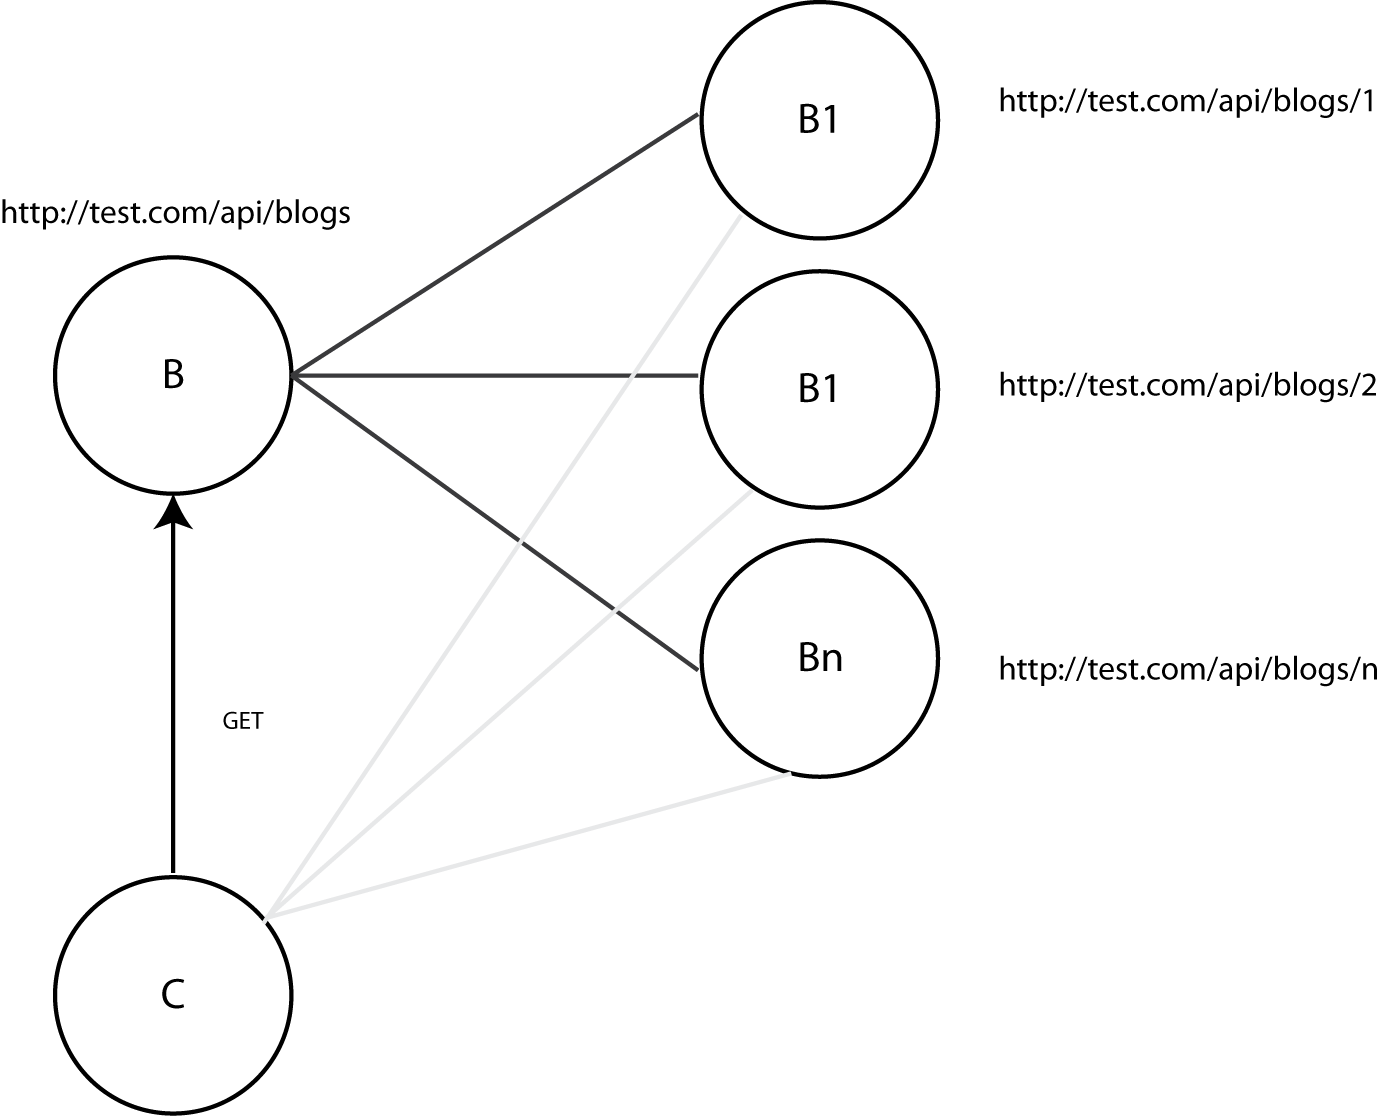
\includegraphics{get_ex.png}
\end{figure}

The symbols used are the following:
\begin{itemize}
  \item Resource $B$ with triple space $TS<B(u)>$ and input channel $l$ with URI \emph{http://test.com/api/blogs}
  \item Client $C$ with triple space $TS<C>$
  \item Type $T$ for the resources of type \emph{http://test.com/api/blog}
  \item Pattern $p$ matching triples of type $T$ in any triple repository
\end{itemize}



\setcounter{equation}{0}
\begin{eqnarray*}
 \ TS<C>,TS<B(u)>\, &\vdash\,&  C\,|\,B(u) \\
 \               &        &          \\
 \ TS<C>,TS<B(u)>\, &\vdash\,& new\,c:[T]\,in\,\overline{l}[GET,p:[T],c:[T]].(rs)c\,|\\
 \               &\,      &(rq)l.[rq = [GET,p_i:[T],c_i[T]]].\overline{c_i}[200,r(u)<p_i>].B(u) \\
 \               &        &          \\
 \ TS<C>,TS<B(u)>\, &\vdash\,& new\,c:[T]\,in\,(rs)c\,|\, \{[GET,p,c]/rq\}.\\
 \               &\,      &[rq = [GET,p_i:[T],c_i:[T]]].\overline{c_i}[200,r(u)<p_i>].B(u) \\
 \               &        &          \\
 \ TS<C>,TS<B(u)>\, &\vdash\,& new\,c:[T]\,in\,(rs)c\,|\, \\
 \               &\,      &[[GET,p,c] = [GET,p_i:[T],c_i:[T]]].\overline{c_i}[200,r(u)<p_i>].B(u) \\
\end{eqnarray*}
\begin{eqnarray*}
\ TS<C>,TS<B(u)>\, &\vdash\,& new\,c:[T]\,in\,(rs)c\,|\,\{p,c/p_i,c_i\} \\
 \               &\,      &\overline{c_i}[200,r(u)<p_i>].B(u) \\
 \               &        &          \\
 \ TS<C>,TS<B(u)>\, &\vdash\,& new\,c:[T]\,in\,(rs)c\,|\,\overline{c}[200,r(u)<p>].B(u) \\
 \               &        &          \\
 \ TS<C>,TS<B(u)>\, &\vdash\,& new\,c:[T]\,in\,(rs)c\,|\,\overline{c}[200,v:[T]].B(u) \\
 \               &        &          \\
 \ TS<C>,TS<B(u)>\, &\vdash\,& \{[200,v]/rs\}\,|\,B(u) \\
 \               &        &          \\
 \ TS<B(u)>\, &\vdash\,& 0\,|\,B(u) \\
\end{eqnarray*}


\subsection{Resource creation}
A client can create new RESTful resources sending the encoded representation of the new resource to a \emph{factory} resource. The new resource will be created by the server and a server chosen URI, under the factory resource URI, will be assigned to it.
In this example, a client send the triple encoded representation of a new resource of type \emph{http://test.com/api/blog} to the factory resource at URI \emph{http://test.com/api/blogs}. The factory resource process creates a new process for the resource, sharing the same triple space, with a new URI under its own URI \emph{http://test.com/api/blogs/3432}, and the channel for the new resource is returned to the client. The triple space for the new process will contain the triple encoded information sent from the client. The triple space of the factory resource will also be updated with the information of the new existent resource.

\begin{figure}[htb!]
\centering%
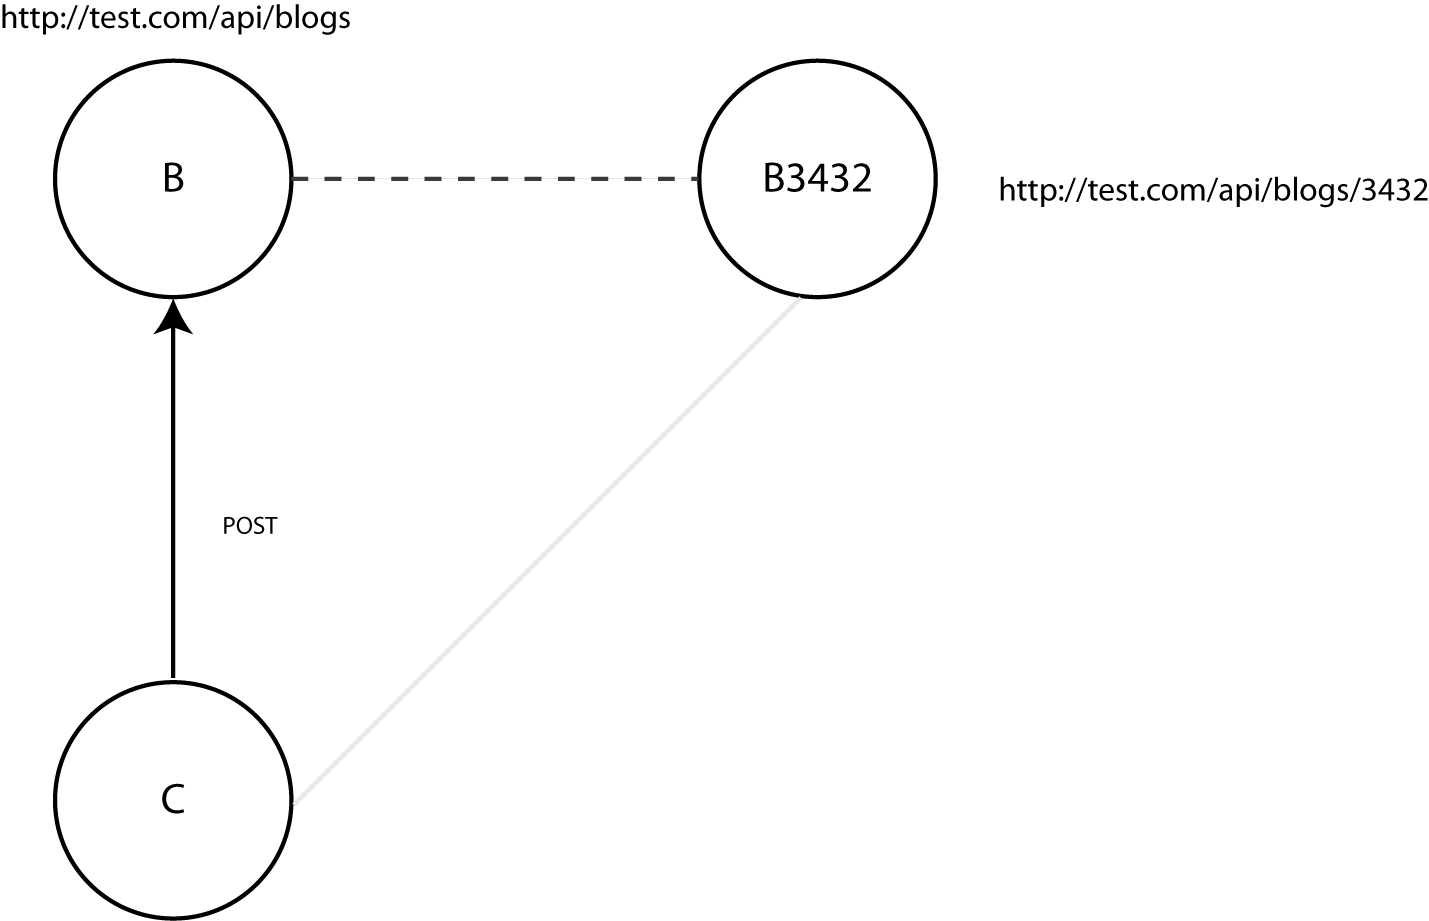
\includegraphics{post_ex.png}
\end{figure}

\setcounter{equation}{0}
\begin{eqnarray*}
 \ TS<C>,TS<B(u)>\, &\vdash\,&  C\,|\,B(u) \\
 \               &        &          \\
 \ TS<C>,TS<B(u)>\, &\vdash\,& new\,c:T\,in\;\overline{l}[POST,p:T,c:T].(rs)c\,|\\
 \               &\,      & new\,r:T\,in\;(rq)l.[rq = [POST,p_i:T,c_i:T]].\\
 \               &        & w(u)<p_i,r>.!B_2(u).\overline{c_i}[201,<p_i,r>].B(u) \\
 \               &        &          \\
 \ TS<C>,TS<B(u)>\, &\vdash\,& new\,c:T\,in\;(rs)c\,|\,new\,r:T\,in\;\\
 \               &\,      & \{[POST,p,c]/rq\}.[rq = [POST,p_i:T,c_i:T]].\\
 \               &        & w(u)<p_i,r>.!B_2(u).\overline{c_i}[201,<p_i,r>].B(u) \\
 \               &        &          \\
 \ TS<C>,TS<B(u)>\, &\vdash\,& new\,c:T\,in\;(rs)c\,|\,new\,r:T\,in\;\\
 \               &\,      & [[POST,p,c] = [POST,p_i:T,c_i:T]].\\
 \               &        & w(u)<p_i,r>.!B_2(u).\overline{c_i}[201,<p_i,r>].B(u) \\
 \               &        &          \\
 \ TS<C>,TS<B(u)>\, &\vdash\,& new\,c:T\,in\;(rs)c\,|\,new\,r:T\,in\;\\
 \               &\,      & \{p,c/p_i,c_i\}.w(u)<p_i,r>.\\
 \               &        & !B_2(u).\overline{c_i}[201,<p_i,r>].B(u) \\
 \               &        &          \\
\end{eqnarray*}
\begin{eqnarray*}
 \ TS<C>,TS<B(u)>\, &\vdash\,& new\,c:T\,in\;(rs)c\,|\,new\,r:T\,in\;\\
 \               &\,      & w(u)<p,r>.!B_2(u).\overline{c}[201,<p,r>].B(u) \\
 \               &        & \\
 \ TS<C>,TS<B(u)>\, &\vdash\,& new\,c:T\,in\;(rs)c\,|\,new\,r:T\,in\;\\
 \               &\,      & w(u)<v:T>.!B_2(u).\overline{c}[201,v:T].B(u) \\
 \               &        & \\
 \ TS<C>,&\vdash\,& new\,c:T\,in\;(rs)c\,|\,new\,r:T\,in\;\\
 \ TS<B(u)>,\cup\{v\}\, &\,      & !B_2(u).\overline{c}[201,v].B(u) \\
 \               &        & \\
 \ TS<C>,TS<B(u)>\, &\vdash\,& new\,c:T\,in\;(rs)c\,|\,new\,r:T\,in\;\\
 \ ,TS<B_2(u)>              &\,      & \overline{c}[201,v].B(u)\,|\,B_2(u) \\
 \               &        & \\
 \ TS<C>,TS<B(u)>,\, &\vdash\,& \{[201,v]/rs\}\,|\,new\,r:T\,in\;\\
 \ TS<B_2(u)>              &\,      & B(u)\,|\,B_2(u) \\
 \               &        & \\
 \ TS<B(u)>,TS<B_2(u)>\, &\vdash\,& 0\,|\,B(u)\,|\,B_2(u) \\
 \               &        & \\
\end{eqnarray*}

\subsection{Resource update}

A client can update any accesible RESTful resource through its URI, sending a new triple encoded representation for the resource in a PUT HTTP request. As a consequence of this request the resource will replace the old triples into its triple space by the new set provided by the client.

\begin{figure}[htb!]
\centering%
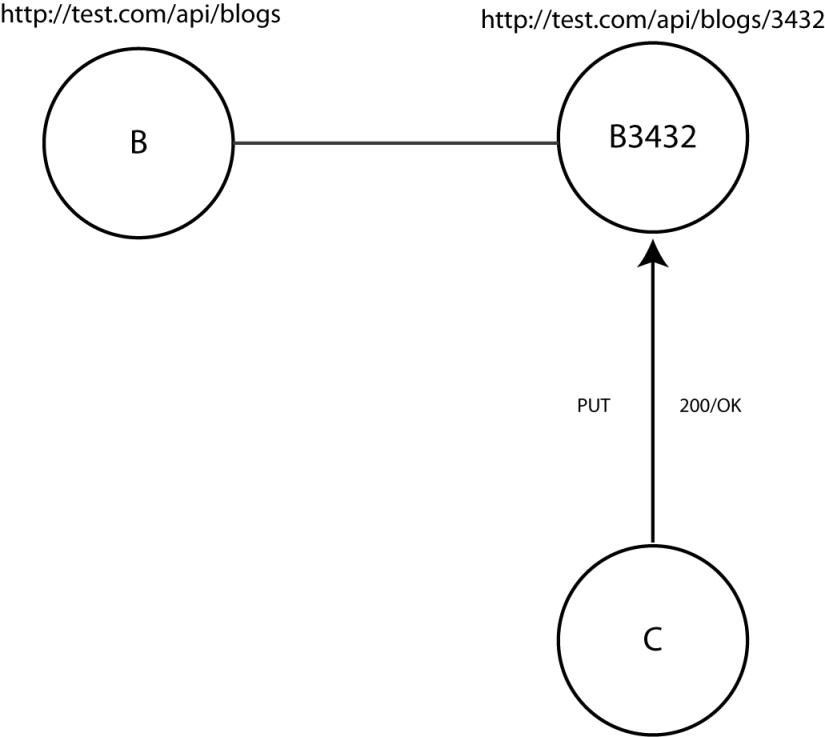
\includegraphics{put_ex.png}
\end{figure}

\setcounter{equation}{0}
\begin{eqnarray*}
 \ TS<C>,TS<B(u)>\, &\vdash\,&  C\,|\,B_2(u)\,|\,B(u) \\
 \ TS<B_2(u)>       &        &          \\
 \               &        &          \\
 \ TS<C>,TS<B(u)>\, &\vdash\,& new\,c:T\,in\;\overline{l}[PUT,v:T,c:T]\,|\\
 \ TS<B_2(u)>       &\,      & (rq)l.[rq = [PUT,v_i:T,c_i:T]].d(u)<r(u)<():T>>.\\
 \               &\,      & .w(u)<v_i>.\overline{c_i}[200,()].B_2(u)\,|\,B(u)\\
 \               &        &          \\
 \ TS<B(u)>,         &\vdash\,& new\,c:T\,in\;0\,|\{[PUT,v,c]/rq\}.\\
 \ TS<B_2(u)>              &\,      & [rq = [PUT,v_i:T,c_i:T]].d(u)<r(u)<():T>>.\\
 \               &\,      & w(u)<v_i>.\overline{c_i}[200,()].B(u)_2\,|\,B(u)\\
 \               &        &          \\
 \ TS<B(u)>,         &\vdash\,& new\,c:T\,in\;0\,|\,[[PUT,v,c]=[PUT,v_i:T,c_i:T].\\
 \ TS<B_2(u)>              &\,      & d(u)<r(u)<():T>>.w(u)<v_i>.\overline{c_i}[200,()].B\\
\end{eqnarray*}
\begin{eqnarray*}
 \               &        &          \\
 \ TS<B(u)>,         &\vdash\,& new\,c:T\,in\;0\,|\,\{v,c/v_i,c_i\}.\\
 \ TS<B_2(u)>              &\,      & d(u)<r(u)<():T>>.w(u)<v_i>.\overline{c_i}[200,()].B_2(u)\,|\\
 \               &        & B(u)\\
 \               &        &          \\
 \ TS<B(u)>,         &\vdash\,& new\,c:T\,in\;0\,|\,\\
 \ TS<B_2(u)>              &      & d(u)<r(u)<():T>>.w(u)<v>.\overline{c}[200,()].B_2(u)\,|\\
 \               &        & B(u)\\
 \               &        &          \\
 \ TS<B(u)>,         &\vdash\,& new\,c:T\,in\;0\,|\,\\
 \ TS<B_2(u)>              &      & d(u)<v_{old}:T>.w(u)<v>.\overline{c}[200,()].B_2(u)\,|\\
 \               &        &  B(u)\\
 \               &        &          \\
 \ TS<B(u)> - \,\{ v_{old} \},        &\vdash\,& new\,c:T\,in\;0\,|\,\\
 \ TS<B_2(u)> - \,\{ v_{old} \}              &      & w(u)<v>.\overline{c}[200,()].B_2(u)\,|\,B(u)\\
 \               &        &          \\
 \ TS<B(u)> \cup \,\{v\},        &\vdash\,& new\,c:T\,in\;0\,|\,\\
 \ TS<B_2(u)> \cup \,\{v\}              &      & \overline{c}[200,()].B_2(u)\,|\,B(u)\\
 \               &        &          \\
 \ TS<B(u)>,TS<B_2(u)>         &\vdash\,& new\,c:T\,in\;0\,|\,\\
 \               &      & \overline{c}[200,()].B_2(u)\,|\,B(u)\\
 \               &       &          \\
 \ TS<B(u)>,TS<B_2(u)>         &\vdash\,& 0\,|\,B_2(u)\,|\,B(u)\\
\end{eqnarray*}


\subsection{Resource destruction}

The destruction of a resource can be achieved by issuing a DELETE HTTP request through the channel identified by the URI of the resource. The resource information will be deleted from the triple space and the process for the resource will terminate.

\begin{figure}[htb!]
\centering%
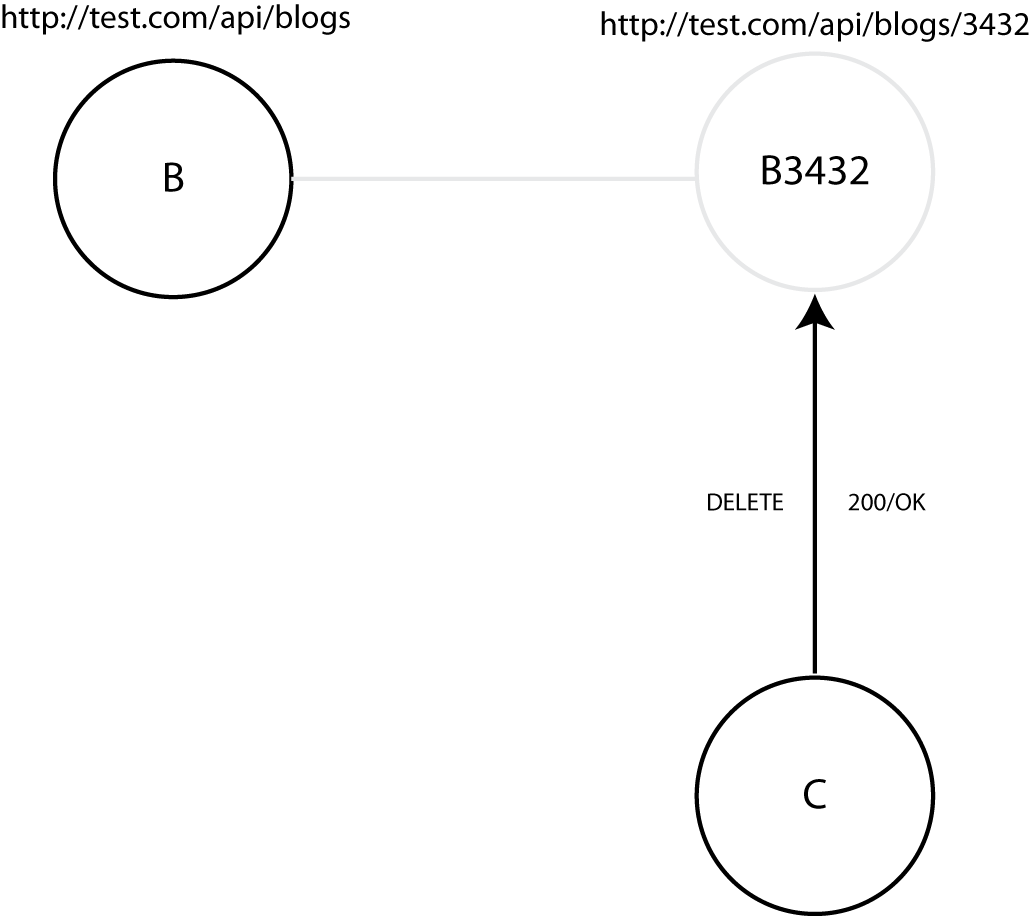
\includegraphics{get_del.png}
\end{figure}

\setcounter{equation}{0}
\begin{eqnarray*}
 \ TS<C>,TS<B_2(u)>\, &\vdash\,&  C\,|\,B_2(u) \\
 \               &        &          \\
 \ TS<C>,TS<B_2(u)>\, &\vdash\,& new\,c:T\,in\;\overline{l}[DELETE,c:T]\,|\\
 \               &\,      & (rq)l.[rq = [DELETE,c_i:T]].d(u)<r(u)<p:T>>.\\
 \               &\,      & \overline{c}[200,()].0\\
 \               &        &          \\
 \ TS<B_2(u)>\, &\vdash\,& new\,c:T\,in\;0\,|\,\{[DELETE,c]/rq\}\\
 \               &\,      & [rq = [DELETE,c_i:T]].d(u)<r(u)<p:T>>.\\
 \               &\,      & \overline{c_i}[200,()].0\\
 \               &        &          \\
 \ TS<B_2(u)>\, &\vdash\,& new\,c:T\,in\;0\,|\,\\
 \               &\,      & [[DELETE,c] = [DELETE,c_i:T]].d(u)<r(u)<p:T>>.\\
 \               &\,      & \overline{c_i}[200,()].0\\
 \               &        &          \\
 \ TS<B_2(u)>\, &\vdash\,& new\,c:T\,in\;0\,|\,\\
 \               &\,      & \{c/c_i\}.d(u)<r(u)<p:T>>.\overline{c_i}[200,()].0\\
 \               &        &          \\
 \ TS<B_2(u)>\, &\vdash\,& new\,c:T\,in\;0\,|\,\\
 \               &\,      & d(u)<r(u)<p:T>>.\overline{c}[200,()].0\\
 \               &        &          \\
\end{eqnarray*}
\begin{eqnarray*}
 \ TS<B_2(u)>\, &\vdash\,& new\,c:T\,in\;0\,|\,\\
 \               &\,      & d(u)<v:T>.\overline{c}[200,()].0\\
 \               &        &          \\
 \ TS<B_2(u)>\,-\,\{v\}\, &\vdash\,& new\,c:T\,in\;0\,|\,\\
 \               &\,      & \overline{c}[200,()].0\\
 \               &        &          \\
 \ &\vdash\,& 0\,|\,0\\
\end{eqnarray*}

\subsection{Clients coordination}

Different client processes sharing the same triple space, can use the blocking operations over the triple space as a mean of coordination in the processing of resources. In this example, there are two process C and D, sharing access to triple space $u_1$, additionally, C has access to triple space $u_2$. C reads a resource P of type T through l, writes it on triple space $u_2$ and on triple space $u_1$. Client D reads the representation of P from $u_1$ and deletes P.
\\
\begin{figure}[htb!]
\centering%
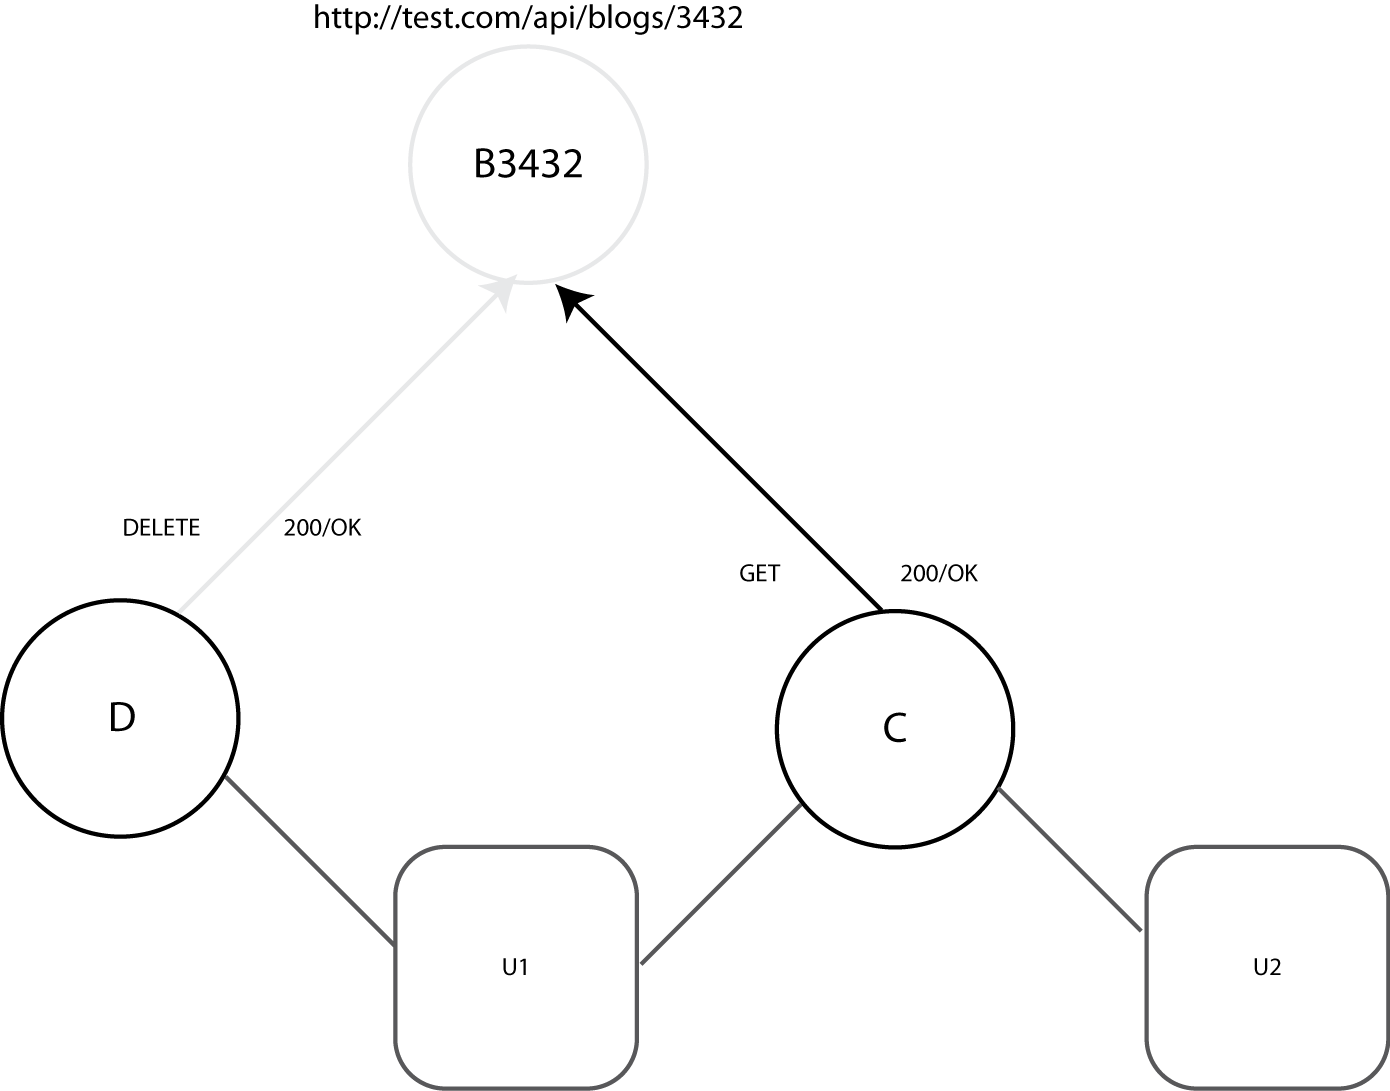
\includegraphics{coord.png}
\end{figure}

\setcounter{equation}{0}
\begin{eqnarray*}
 \ TS<C(u_1,u_2)>,\, &\vdash\,&  P\,|\,C(u_1,u_2)\,|\,D(u_1) \\
 \ TS<D(u_1)>,   &        &          \\
\  TS<P>   &        &          \\
 \               &        &          \\
 \ TS<C(u_1,u_2)>, &\vdash\,& new\,c_1:T,c_2:T,\,in\; (rq)l. \\
 \ TS<D(u_1)>,     &        & [rq = [GET,p_i:T,c_i:T]].\overline{c_i}[200,r<p_i>].P         \\
 \ TS<P>           &        & [rq = [DELETE,(),c_i:T]].d(u)<v_{P}>.\overline{c_i}[200,()].0         \\
 \               &        &    \,|\,      \\
 \               &        &  \overline{l}[GET,p:T,c_1:T].(rs)c_1.[rs = [200,v_o:T]].w(u_2)<v_o>. \\
 \               &        & w(u_1)<v_o>.0        \\
 \               &        &    \,|\,      \\
 \               &        &  br(u_1)<p:T>.\overline{l}[DELETE,(),c_2].0 \\
 \               &        &          \\
 \ TS<C(u_1,u_2)>, &\vdash\,& new\,c_1:T,c_2:T,\,in\; \{[GET,p,c_1]/rq\}. \\
 \ TS<D(u_1)>,     &        & [[GET,p,c_1] = [GET,p_i:T,c_i:T]].\overline{c_i}[200,r<p_i>].P         \\
 \ TS<P>              &        &    \,|\,      \\
 \               &        &  (rs)c_1.[rs = [200,v_o:T]].w(u_2)<v_o>. \\
 \               &        & w(u_1)<v_o>.0        \\
 \               &        &    \,|\,      \\
 \               &        &  br(u_1)<p:T>.\overline{l}[DELETE,(),c_2].0 \\
 \               &        &          \\
 \ TS<C(u_1,u_2)>, &\vdash\,& new\,c_1:T,c_2:T,\,in\; \\
 \ TS<D(u_1)>,     &        & \{ p,c_1 / p_i, c_i \}.\overline{c_i}[200,r<p_i>].P         \\
 \ TS<P>           &        &    \,|\,      \\
 \               &        &  (rs)c_1.[rs = [200,v_o:T]].w(u_2)<v_o>. \\
 \               &        & w(u_1)<v_o>.0        \\
 \               &        &    \,|\,      \\
 \               &        &  br(u_1)<p:T>.\overline{l}[DELETE,(),c_2].0 \\
 \               &        &          \\
\end{eqnarray*}
\begin{eqnarray*}
 \ TS<C(u_1,u_2)>, &\vdash\,& new\,c_1:T,c_2:T,\,in\; \\
 \ TS<D(u_1)>,     &        & \overline{c_1}[200,r<p>].P         \\
 \ TS<P>            &        &    \,|\,      \\
 \               &        &  (rs)c_1.[rs = [200,v_o:T]].w(u_2)<v_o>. \\
 \               &        & w(u_1)<v_o>.0        \\
 \               &        &    \,|\,      \\
 \               &        &  br(u_1)<p:T>.\overline{l}[DELETE,(),c_2].0 \\
 \               &        &          \\
 \ TS<C(u_1,u_2)>, &\vdash\,& new\,c_1:T,c_2:T,\,in\;  \\
 \ TS<D(u_1)>,     &        & \overline{c_1}[200,v:T].P         \\
 \ TS<P>            &        &    \,|\,      \\
 \               &        &  (rs)c_1.[rs = [200,v_o:T]].w(u_2)<v_o>. \\
 \               &        & w(u_1)<v_o>.0        \\
 \               &        &    \,|\,      \\
 \               &        &  br(u_1)<p:T>.\overline{l}[DELETE,(),c_2].0 \\
 \               &        &          \\
 \ TS<C(u_1,u_2)>, &\vdash\,& new\,c_1:T,c_2:T,\,in\; \\
 \ TS<D(u_1)>,   &        & P        \\
 \ TS<P>         &        &    \,|\,      \\
 \               &        & \{[200,v] / rs\}.[rs = [200,v_o:T]].w(u_2)<v_o>. \\
 \               &        & w(u_1)<v_o>.0        \\
 \               &        &    \,|\,      \\
 \               &        &  br(u_1)<p:T>.\overline{l}[DELETE,(),c_2].0 \\
 \               &        &          \\
 \ TS<C(u_1,u_2)>, &\vdash\,& new\,c_1:T,c_2:T,\,in\; (rq)l.[rq = [DELETE,(),c_i:T]].\\
 \ TS<D(u_1)>,   &        & d(u)<v_{P}>.\overline{c_i}[200,()].0         \\
 \ TS<P>              &        & [[200,v] = [200,v_o:T]].w(u_2)<v_o>. \\
 \               &        & w(u_1)<v_o>.0        \\
 \               &        &    \,|\,      \\
 \               &        &  br(u_1)<p:T>.\overline{l}[DELETE,(),c_2].0 \\
 \               &        &          \\
\end{eqnarray*}
\begin{eqnarray*}
 \ TS<C(u_1,u_2)>, &\vdash\,& new\,c_1:T,c_2:T,\,in\; (rq)l.[rq = [DELETE,(),c_i:T]].\\
 \ TS<D(u_1)>,   &        & d(u)<r(u)<p_i:T>>.\overline{c_i}[200,()].0         \\
 \ TS<P>         &        &    \,|\,      \\
 \               &        & \{v / v_o \}.w(u_2)<v_o>.w(u_1)<v_o>.0 \\
 \               &        &    \,|\,      \\
 \               &        &  br(u_1)<p:T>.\overline{l}[DELETE,br(u_1)<p:T>,c_2].0 \\
 \               &        &          \\
 \ TS<C(u_1,u_2)>, &\vdash\,& new\,c_1:T,c_2:T,\,in\; (rq)l.[rq = [DELETE,(),c_i:T]].\\
 \ TS<D(u_1)>,   &        & d(u)<r(u)<p_i:T>>.\overline{c_i}[200,()].0         \\
 \ TS<P>         &        &    \,|\,      \\
 \               &        & w(u_2)<v>.w(u_1)<v>.0 \\
 \               &        &    \,|\,      \\
 \               &        &  br(u_1)<p:T>.\overline{l}[DELETE,(),c_2].0 \\
 \               &        &          \\
 \ TS<C(u_1,u_2)>\,\cup\,\{v\}, &\vdash\,& new\,c_1:T,c_2:T,\,in\; (rq)l.[rq = [DELETE,(),c_i:T]]. \\
 \ TS<D(u_1)>,   &        & d(u)<r(u)<p_i:T>>.\overline{c_i}[200,()].0         \\
 \ TS<P>         &        &    \,|\,      \\
 \               &        & w(u_1)<v>.0 \\
 \               &        &    \,|\,      \\
 \               &        &  br(u_1)<p:T>.\overline{l}[DELETE,(),c_2].0 \\
 \               &        &          \\
 \ TS<C(u_1,u_2)>\,\cup\,\{v\}, &\vdash\,& new\,c_1:T,c_2:T,\,in\; (rq)l.[rq = [DELETE,(),c_i:T]]. \\
 \ TS<D(u_1)>,   &        & d(u)<r(u)<p_i:T>>.\overline{c_i}[200,()].0         \\
 \ TS<P>         &        &    \,|\,      \\
 \               &        & 0 \\
 \               &        &    \,|\,      \\
 \               &        &  br(u_1)<p:T>.\overline{l}[DELETE,(),c_2].0 \\
 \               &        &          \\
 \ TS<D(u_1)>, &\vdash\,& new\,c_1:T,c_2:T,\,in\; (rq)l.[rq = [DELETE,(),c_i:T]].\\
 \ TS<P>   &        & d(u)<r(u)<p_i:T>>.\overline{c_i}[200,()].0         \\
 \         &        &    \,|\,      \\
 \               &        & 0 \\
 \               &        &    \,|\,      \\
 \               &        &  br(u_1)<p:T>.\overline{l}[DELETE,(),c_2].0 \\
 \               &        &          \\
\end{eqnarray*}
\begin{eqnarray*}
 \ TS<D(u_!)>, &\vdash\,& new\,c_1:T,c_2:T,\,in\; (rq)l.[rq = [DELETE,(),c_i:T]]. \\
 \ TS<P>   &        & d(u)<r(u)<p_i:T>>.\overline{c_i}[200,()].0         \\
 \         &        &    \,|\,      \\
 \               &        & 0 \\
 \               &        &    \,|\,      \\
 \               &        & br(u_1)<v>.\overline{l}[DELETE,(),c_2].0 \\
 \               &        &          \\
 \ TS<D(u_1)>, &\vdash\,& new\,c_1:T,c_2:T,\,in\; (rq)l.[rq = [DELETE,(),c_i:T]]. \\
 \ TS<P>   &        & d(u)<r(u)<p_i:T>>.\overline{c_i}[200,()].0         \\
 \         &        &    \,|\,      \\
 \               &        & 0 \\
 \               &        &    \,|\,      \\
 \               &        & \overline{l}[DELETE,(),c_2].0 \\
 \               &        &          \\
 \ TS<P> &\vdash\,& new\,c_1:T,c_2:T,\,in\; \{[DELETE,(),c_2] / rq \}. \\
 \    &        & [rq = [DELETE,(),c_i:T]].d(u)<r(u)<p_i:T>>.\overline{c_i}[200,()].0         \\
 \         &        &    \,|\,      \\
 \               &        & 0 \\
 \               &        &    \,|\,      \\
 \               &        & 0 \\
 \               &        &          \\
 \ TS<P> &\vdash\,& new\,c_1:T,c_2:T,\,in\; [[DELETE,(),c_2] = [DELETE,(),c_i:T]].\\
 \    &        & d(u)<r(u)<p_i:T>>.\overline{c_i}[200,()].0         \\
 \         &        &    \,|\,      \\
 \               &        & 0 \\
 \               &        &    \,|\,      \\
 \               &        & 0 \\
 \               &        &          \\
 \ TS<P> &\vdash\,& new\,c_1:T,c_2:T,\,in\; \\
 \    &        & \{c_2 / c_i\}.d(u)<r(u)<p_i:T>>.\overline{c_i}[200,()].0         \\
 \          &        &    \,|\,      \\
 \               &        & 0 \\
 \               &        &    \,|\,      \\
 \               &        & 0 \\
\end{eqnarray*}
\begin{eqnarray*}
 \               &        &          \\
 \ TS<P> &\vdash\,& new\,c_1:T,c_2:T,\,in\; \\
 \   &        & d(u)<v>.\overline{c_2}[200,()].0         \\
 \          &        &    \,|\,      \\
 \               &        & 0 \\
 \               &        &    \,|\,      \\
 \               &        & 0 \\
 \               &        &          \\
 \ TS<P>\,-\,\{v\} &\vdash\,& new\,c_1:T,c_2:T,\,in\; \\
 \    &        & \overline{c_2}[200,()].0         \\
 \         &        &    \,|\,      \\
 \               &        & 0 \\
 \               &        &    \,|\,      \\
 \               &        & 0 \\
 \               &        &          \\
 \  &\vdash\,& new\,c_1:T,c_2:T,\,in\; \\
 \    &        & 0         \\
 \         &        &    \,|\,      \\
 \               &        & 0 \\
 \               &        &    \,|\,      \\
 \               &        & 0 \\
 \               &        &          \\
\end{eqnarray*}

\section{Extensions}
Some possible extensions to easily model some aspects of the services consumption process are discussed in this section.

\subsection{Headers and authentication}
In RESTful architectures, HTTP protocol headers are used along with the request and response bodies to exchange useful information between clients and servers. In the proposed version of the calculus, the only use of headers has been the returning of a response code from the server process.\\
It may be interesting to include support for including collection of headers in the messages exchanged between processes. We could define the messages as:\\
\begin{equation*}
m\,::=\,[VERB,[(k,v)]:[H],v:T,c:T]
\end{equation*}
\\Where $[(k,v)]$ is a collection of headers with keys $k$ and value $v$. The information sent in the headers of the request can be used to define primitives for authentication or conditional request.

\subsection{Metaresources}
In the proposed calculus types have been used to add aditional information to the channels, patterns and messages exchanged. Information about these types are provided beforehand something that is not a realistic assumption for actual implementations of the calculus, where clients will need some kind of mechanism to retrieve the type associated to the URIs and triples returned from these URIs. A possible solution to this problem is the definition of special resources capable of describing other resources, offering information about the types of the resources described, channels and operations available on them.\\
The formalization of these metaresources can be achieved extending the calculus with some extra syntax:
\begin{itemize}
  \item $r:R<T>$: a set of triples describing a resource of type $T$.
  \item $<r:R<T>,v:T>$: applying a description of type $T$ to a resource of type $T$.
\end{itemize}
The result of applying the description to a resource is a set of datatype properties and object properties, where the object properties, consisting on typed URIs, can be used by the client to retrieve related resources.

\section{Conclusions}
In this document a formal system for describing RESTful web servies and the interaction between clientes and servers has been described. The calculus describes what we call semantic RESTful web services since all the representation of resources and communication channels are typed offering metainformation about the resources offered. The calculus is also based on ideas extracted from triple space computing offering a common representation for the values exchanged and communication operations between processes based on triple spaces. Each resource representation is retrieved or sent as sets of triples or patters for triples retrieval and each process has one or more associated triple spaces where these triples are stored and modified.\\
The calculus proposed can be useful when addressing important theoretical questions about distributed systems based on RESTful web services such as whether two systems are equivalent.\\
The calculus can also serve as the solid foundation for a software implementation of a system capable of automating the building and composition of RESTful web services.



\chapter{Technical Specification of RESTful Semantic Web services }\label{capituloTS}

\section{Introduction}

In the previous chapter of this document (\ref{capituloFD}) we have introduced a formal theoretical model allowing the description of
semantic restful web services. In this chapter we wil transform this theoretical model in a technical specification
allowing the practical implementation of such a formal model.\\
In this effort great care has been taken into using actual web standards for semantic technologies as well as for the
description of web services. The use of open standards in the specification of a RESTful semantic web services layer
allows easy reusing of existent technologies and software libraries already deployed in present day HTTP agents like web
browsers, ensuring interoperability.\\
The final output of this chapter will be technical description specifying  how to use different existing web standards to
leverage semantic RESTful web services.  In this specification  the following parts of the formal model
must be present:
\begin{itemize}
\item It must specify how to expose the triples containing the meta data of the resource exposed as a RESTful
  semantic web service.
\item It must specify the necessary meta data for a client being able to access the resource through the HTTP uniform
  interface.
\item It must provide a mechanism to transform the resource triplets representation into a concrete syntax in order for clients and
  services to exchange triples through the HTTP uniform interface.
\end{itemize}

One of the main advantages of the REST architectural point of view in the description of web services is its
simplicity. As we have mentioned, this focus on simplicity has been perceived as a reaction to the complexity in the
specification of WS-* style web services. REST principles avoid complexity restricting the expresiveness in the
description of web services to the design principles of the HTTP protocol. Unfortunately, the HTTP protocol  does not include any
standard way to add semantics to the data exchanged through the protocol. In our specification we have tried to add the
minimum necessary overhead on top of REST so these metadata can be automatically exchanged by web agents while staying true to the
simplicity and principles of the HTTP protocol. When dealing with semantic metadata, the main point of interest is the automatic processing of these semantic metadata. We believe  the necessity of automatic processing of the semantic information justifies the use of description languages in a RESTful way, for instance, as metaservices describing the semantics of other services.

\section{State of the Art}
In the world of WS-* web services there has been a great deal of effort in creating effective ways of describing web
services as well as the mechanisms of interaction between services and clients. Standards such as the Web Services
Description Language (WSDL) \cite{w3cwsdl}
offer languages for writing service descriptions that can be automatically processed by client software in order to
generate the necessary code to consume the service.\\
The first version of the WSDL 1.1 specification bindings to the HTTP protocol were inadequate, preventing thus the
description of RESTful web services using this standard. The situation has change with the version 2.0 of the standard
\cite{w3cwsdl2} there have been and improvement of the HTTP bindings allowing the description of WS-* web services with
REST semantics.\\
Outside the standardization efforts of the W3C there have been other proposals fo HTTP based web services description
languages like WADL \cite{wadl}. The main focus of the WADL proposal is in the automatic generation of client code for
accesing the the services resources,  but it has been received with mild
enthusiasm from the RESTful web services developer community and no great adoption of the technology has followed. \\
Main criticism against proposals as the Web Application Description Language (WADL) \cite{greg2007} has come from the observation of the
fact that the complexity in description languages contrast with the alleged simplicity of RESTful web services,
concernings about the RESTful nature of these mechanisms and a perceived lack of sustantial gains in the adoption of the
code generation technologies these languages could enable.\\

In parallel with the advances in the standardization of description languages for web services and RESTful web services,
the W3C semantic web initiative has been fruitful in the generation of standards for the description of semantic
metadata on the web.\\

The foundation of the semantic technologies from the W3C is the Resource Description Framework (RDF) specification \cite{Hayes:04:RS}. RDF describes a
data model allowing anyone ot insert into a HTTP accesible resources assertions about any other web resource designated
after its URI. The resources linked through this assertions conforms a graph of resources that RDF serializes as a set
of triples with subject, predicate and object. This graph can also be serialized, for instance,  as an XML document \cite{rdfxml} and
exposed as a web resource with its own URI. RDF serves as a good foundation for adding simple semantic
descriptions. More complex and expressive ways of adding metadata  have been proposed later as new specifications built
on top of the RDF data model. These specifications were aimed at the specification of ontologies for web resources
allowing inference. The
first of these standard is RDF Schema \cite{Brickley:04:RVD} which provides a set of ontological primitives that can be
annotated to web resources using the RDF data model. The limited expresiveness of RDF Schema lead to the proposal of the
Ontolgy Web Language (OWL) \cite{Dean:04:OWO} in its three version OWL Lite, Full and DL. These last specification has
its roots in the field of description logics and offers a vocabulary for the building of ontologies around web
resources, with well defined semantics.\\

The standardization of these semantic technologies has made possible a whole new kind of software applications in recent
years and has obtained a considerable success. Its adoption nevertheless has not reached its full extent. In a way that
resembles the situtaion happened with WS-* specifications, many users have perceived specifications as OWL as too complex for
use cases not involving inference. Independent proposals for adding semantic metadata into web resources have appeared,
the one meeting the most success being the Microformats initiative. Microformats are small patterns of HTML describing
common entties in the web. They try to provide some of the benefits that can be obtained from the use of the standard
semantic languages avoiding its complexity. The microformats ad-hoc nature nevertheless presents several important drawbacks,
like the lack of a formal model for the description, or the unability to use name spaces in the descriptions.\\

In spite of its limitations, the microformats proposal has met a certain degree of success between web application
developers, helping to bridge the gap between the standar semantic technologies and the web application developers
community. This success has motivated in the last months that the W3C standarized Annotated RDF (RDFa)  \cite{rdfa} as
a standard way of inserting RDF graphs into HTML pages. Support for the indexing of microformats and RDFa documents has
been announced by different search engines companies as Google.\\

Web services and semantic web standards have had a confluence in recent work in the technical specification of a
semantic web services specification language. Between the different proposals submitted for their standarization to the
W3C we can found the  Web Service Modeling Ontology (WSMO) \cite{wsmo}, Semantic Markup for Web Services (OWL-S) \cite{owls}.\\ 
WSMO is the most evolved specifcation, related to sub projects as the Web Service Modeling Langauge (WSML) \cite{wsml}
and the Web Service Modelling Execution Environment \cite{wsmx}. This set of specifications provides a reference model
(WSMO), a syntax (WSML) and a standard implementation (WSMX) of the necessary technologies for specifying and building
semantic web services. In the other hand, OWL-S provides an alternative model for the description of semantic web
services but relies in the standard mechanisms of OWL for the specification of the elements of the service instead of
creating a new one as WSMO does with WSML. \\

Both specifications provide rich models for the description of semantic web services. These conceptual models needs to
be transformed into an exchange syntax and transmitted through a communication channel using a certain communication
protocol, so the information contained in these model can be exchanged between agents. The problem of solving this
abstraction gap is known as grounding into service oriented architectures jargon. The main aspects of web services
grounding can be splitted into data grounding and behavioural grounding \cite{ISBN:3540345191}. Data grounding
transforms the information retrieved from the service into a serialization format. WSMO and OWL-S uses XML as the
encoding  of these messages. Behavioural grounding provides the information necessary for a client to know how to invoke
a service and what kind of messages it should send and receive. WSMO and OWL-S provide their own solution for this
problem involving an interaction model, an abstract state machine in the cas of WSMO, and some XML encoded information
about the kind of messages that can be sent in and out of the service. OWL-S tries to reuse the existent WS-*
techologies providing a mapping from its conceptual model to these technologies. The same approach has been followed by
other W3C submission proposals as the Semantic Web Services Description Language (WSDL-S) \cite{wsdls} consisting in
a lightweight layer of semantic annotations for the components of WSDL.

Up to this point the main poposals for semantic web services have been reviewed. We have noted how they try to join the
world of WS-* web services and W3C standards for the semantic web. We have also taken into account how these standards
have sometimes met criticism for their complexity and have been found unsuitable for certain kind of applications,
spawning lightweight approachs to the same problems as is the case of REST for web services and the microformats
initiative in the case of the W3C standards. We have also seen how this simpler proposals have been integrated in
different ways into the standards as is the case of WSDL 2.0 for WS-* web services and RDFa for semantic metadata.\\

In the world of semantic web services, similar provisions about the complexity of the technologies have started to be
taken. Most notably WSMO has produced reduced versions of the WSMO standard aiming to reduce its complexity: WSMO Lite
\cite{wsmolite} and MicroWSMO \cite{microwsmo}.\\

Both working drafts sketch a reduced WSMO model suitable for simpler web services. MicroWSMO is of an special interest
due to the reason that it tries to adapt the WSMO model to the construction of RESTful semantic web services. As a
complement of the MicroWSMO minimal model another specification knowns as hRESTS has been drafted proposing a vocabulary
expressed as a microformat or a RDFa encoded set of WSML statements for the description of MicroWSMO semantic web
services. \\

From this point of view MicroWSMO/hRESTS is similar to other mechanisms for extracting metadat from a HTML web resource
attaching a transformation mechanism, as the W3C recommendation Gleaning Resource Descriptions from Dialects of
Languages (GRDDL) \cite{Connolly:07:GRD}\\

In this document we will use the MicroWSMO/hRESTS standard proposal, as the basis of our technical description of RESTful semantic web services.

\section{hRESTS description mechanism}

The main aim of hRESTS is to offer a simple way of describing RESTful web services semantics. The ease of use of hRESTS originates in the minimality of the service model described, which has only four basic elements:

\begin{enumerate}
  \item service: the RESTful web services being described
  \item operation: the action that a client can perform in the server
  \item input message: the information sent to the service when performing an operation
  \item output message: the information received from the service after an operation is performed
\end{enumerate}

Each operation is described using the HTTP uniform interface stating the HTTP method and an address consisting of an URL template. This information is asserted as a RDF graph, reusing the vocabulary of the WSMO-Lite semantic web services framework.

\subsection{semantic information in hRESTS}
Semantic metadata are added to the service description in hREST through the description of input and output messages. These elements of the service model allow the assertion of the model of the resource being retrieved or modified.\\
Within the model information there are also links to the description of the necessary transformations to translate the information of the data model into the syntax of the message exchanged between client and server. These transformations are known as lowering (from the model to the exchange syntax) and lifting (from the exchange syntax to the model).

\begin{figure}[htb!]
\centering%
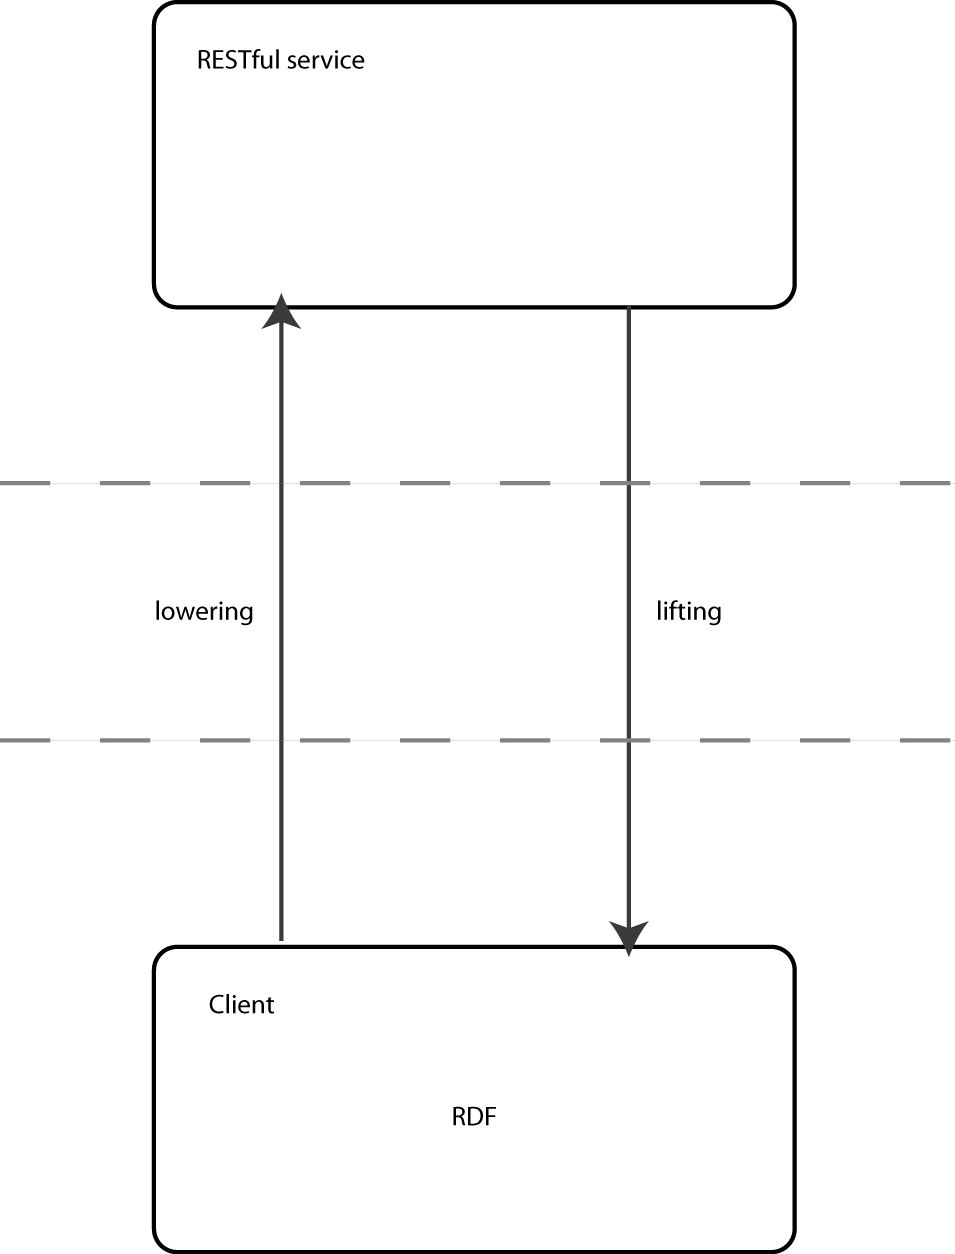
\includegraphics{lifting_lowering.png}
\end{figure}

hRESTS does not specifies a mandatory mechanism for lifting and lowering resources, but offers a mechanism to link the description of the transformations into the service description.

\subsection{encoding of hRESTS descriptions}
A valid hRESTS service description is a RDF graph and thus can be encoded in different formats. All these formats are equivalent for a hRESTS service description, but the proposed encodings for hREST are based in the encoding of the service RDF graph into plain HTML documents. The use of annotated HTML descriptions is the preferred way of describing actual RESTful web services. hRESTS proposes the use of a microformat for inserting the RDF information in these documents. Another proposed mechanism is the use of RDFa \cite{rdfa}, a new W3C standard that makes easy the insertion of RDF graphs inside of XHTML documents.\\
Both encodings have advantages and disadvantages. The use of microformats is a well stablished way of addig semantic information in the development of web applications, and it has big support from the RESTful services community, although it lacks normative recognition and does not have support for namespaces. RDFa on the other hand, is a standard proposal backed by the W3C and also has support for namespaces, but lacks adoption and browse support.\\
Other encodings for hRESTS RDF graphs as YAML and JSON, not covered in the original hRESTS work are explored in this chapter.

\section{hRESTS Grounding}
In this paper a possible grounding mechanism for semantic RESTful web services will be described. \emph{Grounding} is the part in any web services architecture, acting as link between semantic and syntactic descriptions of web services \cite{ISBN:3540345191}, and in the case of \emph{data grounding} how the syntax of a message containing  a representation for that service can be transformed into its semantic counterpart or the other way round.\\
Both transformations, from syntactic representation to semantic representation and from semantic representation to syntactic representation, are commonly called \emph{lifting} and \emph{lowering} as in the W3C recommendation: 'Semantic Annotations for WSDL and XML'' (SAWSDL)  \cite{Lausen:07:SAW}. Lifting and lowering operations present a major difficulty in the specification of semantic web services architectural models. Frameworks like WSMO \cite{wsmo} or OWL-S  \cite{owls} have addressed this issue in different ways. Most of these solutions involve a mixture of XML transformation technologies like XSLT, with web services specific recommendations like WSDL \cite{w3cwsdl} or the aforementioned SAWSDL. Other technologies like XPath \cite{xpath} and XQuery \cite{xquery} are also used. There are  W3C standards like GRDDL (Gleaning Resources Descriptions from Dialects of Languages) \cite{Connolly:07:GRD} specifically created to ease the burden of the tranformation between XML syntactic description of a service and its RDF representation in the semantic model. Other non standardised proposals such as XSPARQL \cite{xsparql} has been created seeking to offer more flexible mechanisms for the translation between XML and RDF.\\
Most of these standards are complex specifications created in the tradition of existing WS-* description mechanisms. They can be used as useful grounding mechanisms for the description of semantic RESTful web services but the particular characteristics of this kind of web services would make desirable a lighter and simpler mechanism for RESTful web services grounding. This paper aims to describe such a mechanism, built over the foundation of existing web grounding technologies.\\

\section{Existent semantic web services grounding mechanisms}
In this section the main existing alternatives for the grounding of semantic web services will be briefly reviewed

\subsection{SAWSDL, WSDL2.0 and HTTP Binding}
WSDL2.0 describes a possible binding for the WSDL components of operation, input and output messages to HTTP concepts \cite{w3cwsdl2}. The following devices are used:
\begin{itemize}
  \item HTTP request IRI location is used as a template for input message in a WSDL operation
  \item HTTP headers are used as a possible binding for the input and output messages of a WSDL operation
  \item Selection of an encoding mechanism for the input and output messages between application/x-www-form-urlencoded, multipart/form-data and application/xml
\end{itemize}
These WSDL concepts and their HTTP bindings can be decorated with SAWSDL annotations. These annotations identify the semantic model involved in the WSDL operation and the transformation mechanisms between the XML representation of the service and the semantic model. SAWDSL does not enforce a certain semantic modelling language. The only requirement made is that concepts from the semantic model should be identified by an IRI. In the same way, any transformation mechanism can be associated to the input and output components of WSDL throught the lifting and lowering constructs of SAWDL. Possible transformation mechanisms are XSLT, XQuery, SPARQL \cite{sparql} or XSPARQL \cite{xsparql}.
In figures 1 to 3, conceptual relations between the different standards used in the grounding mechanism, from HTTP to SAWSDL, are shown.

\begin{figure}[htb!]
\centering%
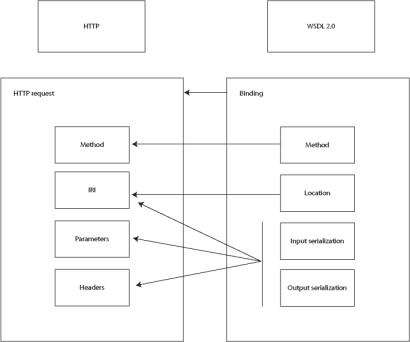
\includegraphics{wasdl1.png}
\caption{WSDL to HTTP mapping}
\end{figure}

\begin{figure}[htb!]
\centering%
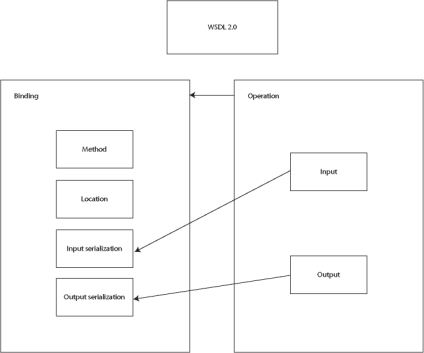
\includegraphics{wasdl2.png}
\caption{WSDL to WSDL HTTP binding}
\end{figure}

\begin{figure}[htb!]
\centering%
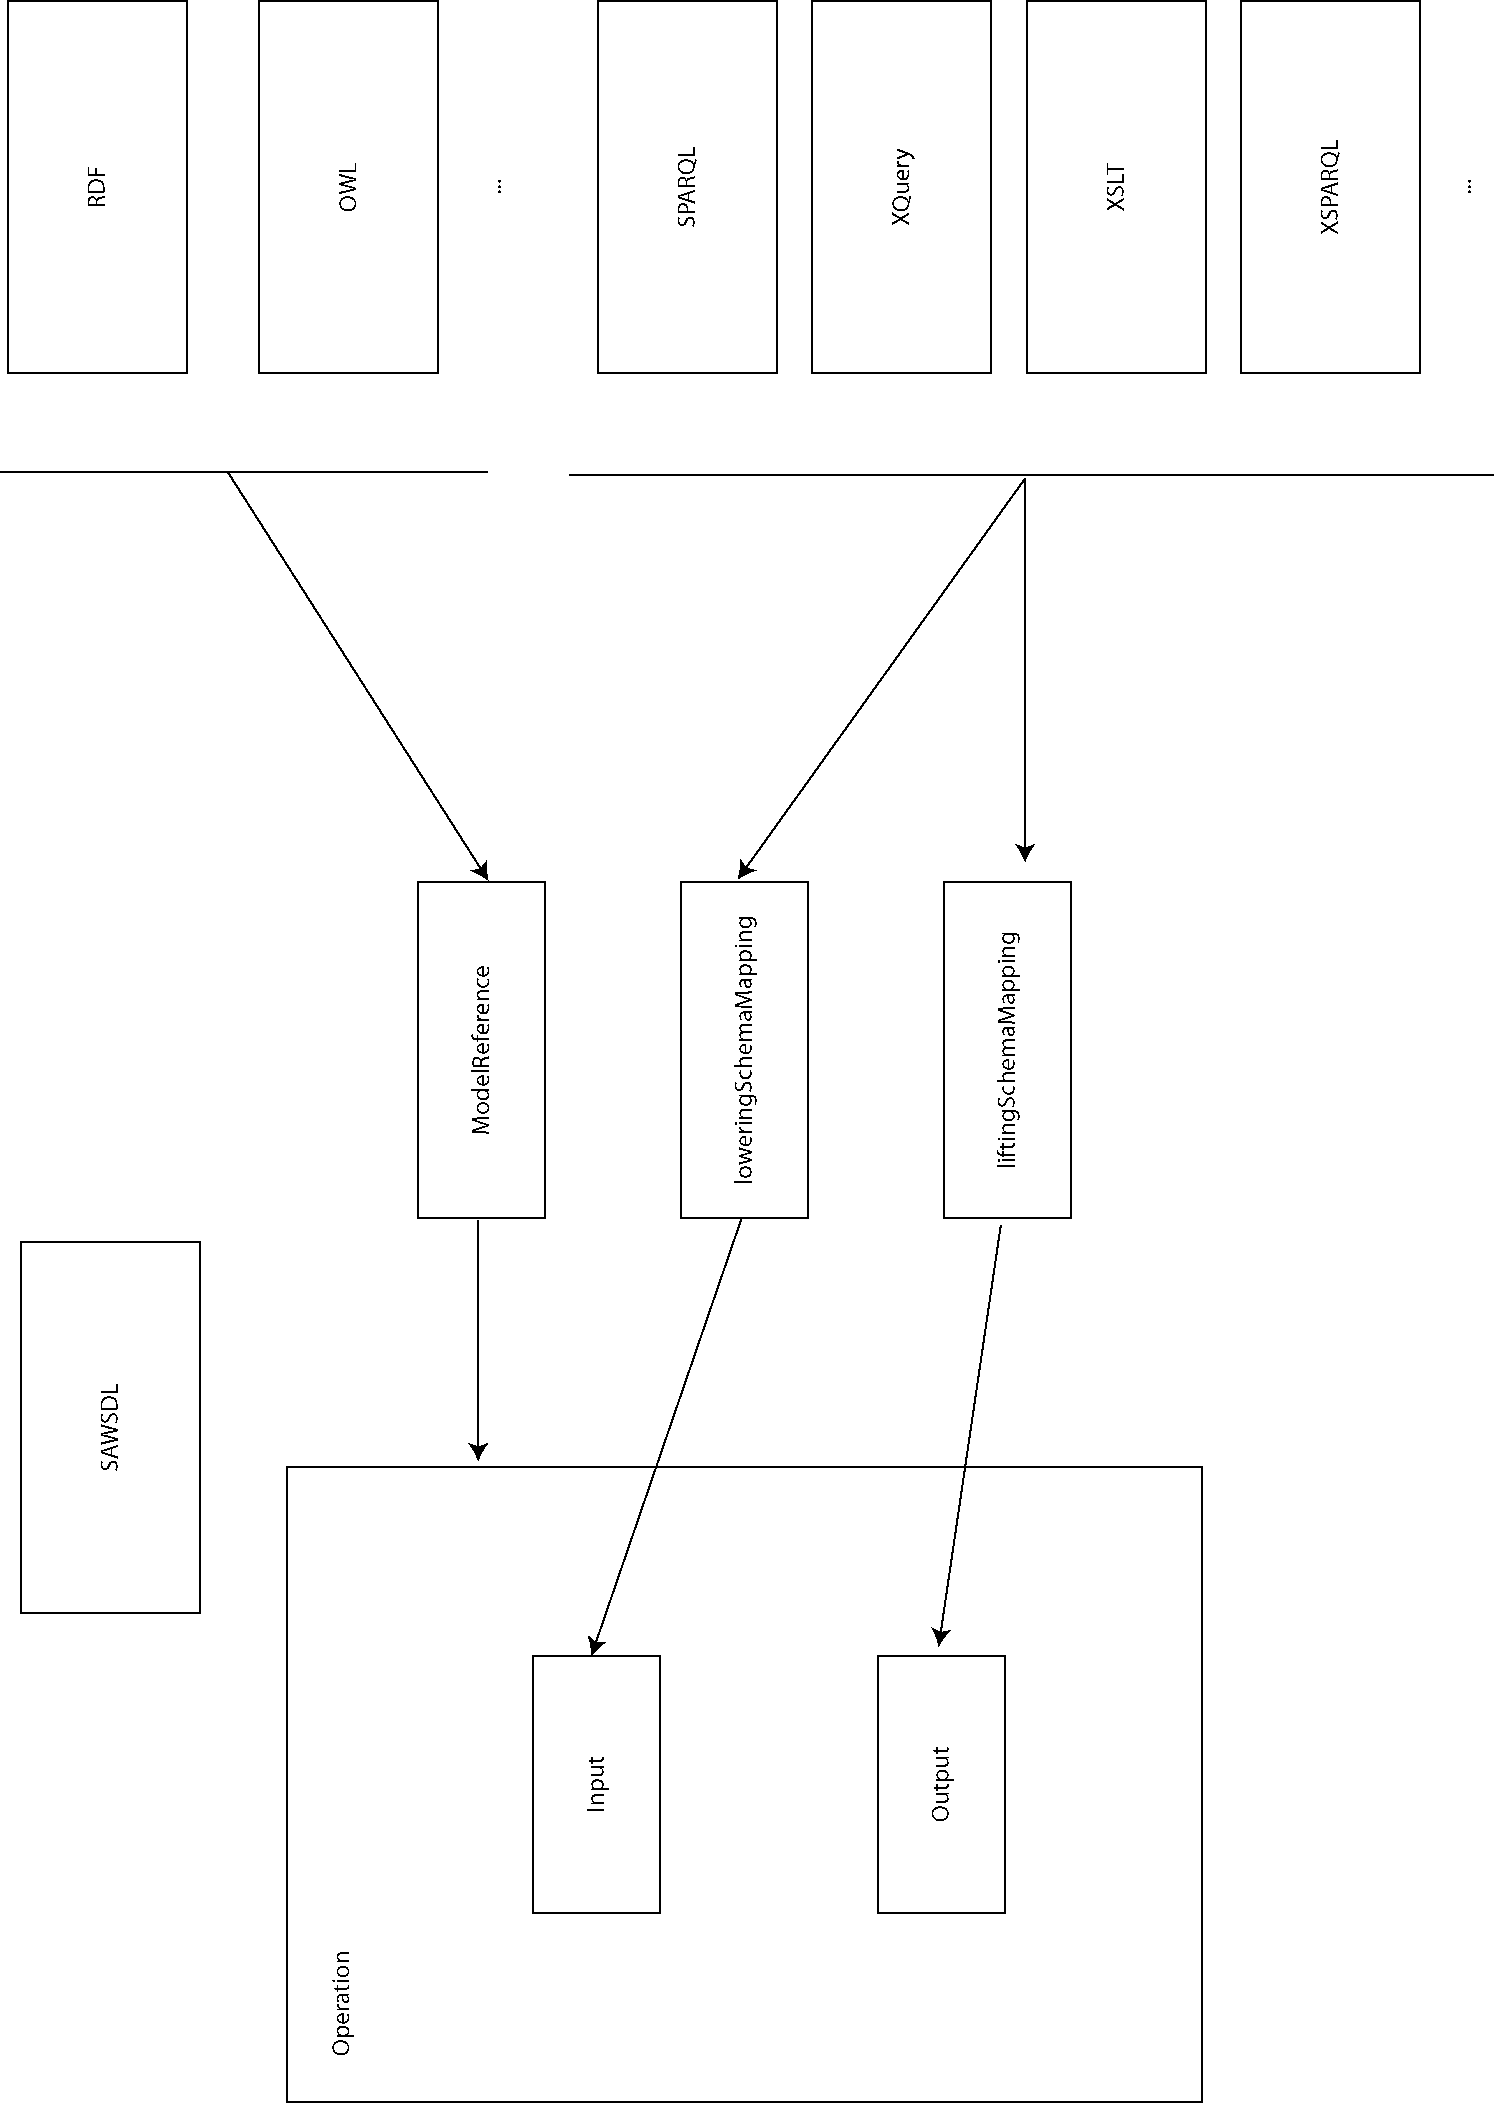
\includegraphics{wasdl3.png}
\caption{SAWSDL annotations}
\end{figure}

\subsection{WSMO Lite and OWL-S}
WSMO Lite \cite{wsmolite} has been conceived as a semantic layer over WSDL but no grounding mechanism is included into WSMO Lite. The ontology for describing semantic web services in WSMO Lite can be transformed into WSDL by means of an annotations mechanism. SAWSDL is proposed as the chosen mechanism but any other semantic annotations language could be used.\\
In the case of OWL-S, this semantic ontology for web services is situated in a similar conceptual relation to WSDL as WSMO Lite. Nevertheless, in this case, the annotation mechanism is included in the ontology vocabulary. This is accomplished by the insertion of OWL-S WsdlGrounding class instances. These elements define XSLT transformations for the input and output messages of WSDL.

\subsection{Transformation languages}
As we have seen, every grounding specification ultimately relies on a transformation mechanism describing how an original model must be transformed into a destination model. The original and destination models can be the semantic model of the object or the returned XML description of the data retrieved. There exists different standard models to describe such transformations, like XSLT or XQuery. All these technologies are complementary and can be used together to obtain more expressive tranformation models.

\begin{itemize}
\item \bf{XSLT}
\end{itemize}

XSLT \cite{xslt} describes a set of constructs arranged in a stylesheet to tranform in a functional fashion XML documents into different XML documents. XSLT can be used in a lowering operation to transform a XML document containing a serialization of a RDF graph into a XML document with the syntax accepted by the service. For lifting operations the XML document returned from the service could be transformed by a XSLT stylesheet into XML/RDF.\\
The support for XSLT is quite mature and every major web browser has support for XSLT tranformations.

\begin{itemize}
\item \bf{XPath}
\end{itemize}

XPath is a standard language which allows the user to specify selections of certain parts in a XML document. XPath grants a set of operations and basic functions that can be applied to path expressions to match parts of the XML document. XPath alone cannot be used as a lifting and lowering mechanism, but it is a basic building block for different transformation languages like XSLT. The current support for XPath in browsers and other tools is fairly good and mature implementations of the standar are available.

\begin{itemize}
\item \bf{XQuery}
\end{itemize}

XQuery is a full programming language, embeddable in XML documents, that allows the retrieval of parts of a document, its transformation, and the creation of new XML documents based on the processed data. XQuery overlaps to a certain degree with XSLT, but while XSLT is a stylesheet language XQuery was conceived as a more general language for retrieving and processing information from other sources than XML documents, like SQL databases. There are numerous implementations of XQuery, but the complexity of the language currently prevents its implementation in many applications like commercial browsers. XQuery can be used alone to specify any kind of transformation in the lifting and lowering operations of a web service.

\begin{itemize}
\item \bf{SPARQL}
\end{itemize}

SPARQL is the standard way of retrieving triplets from RDF graphs. It offers a query language similar to SQL where variables are declared along with query modifiers. As a result, a set of bindings for those variables is obtained from the RDF repository or graph when the query is processed. SPARQL also offers constructs to build new graphs from SPARQL queries. SPARQL can be used in combination with a tranformation language to offer a complete lifting and lowering mechanism.

\begin{itemize}
\item \bf{XSPARQL}
\end{itemize}

XSPARQL is a recent proposal for a transofmation mechanism specifically conceived to ease the tranformation between RDF and different XML formats. It has been conceived  with lowering and lifting operations necessities in mind. XSPARQL can be described as a mixture of SPARQL query capabilities with the XQuery syntax. The flexibility of SPARQL allows a easier retrieval of information from RDF graphs that can be later processed with XQuery constructs. These features made up for a powerful lifting and lowering mechanism. Nevertheless, XSPARQL hast not been yet submitted as a recommendation proposal and its support by tools is almost non existent.

\begin{itemize}
\item \bf{GRDDL}
\end{itemize}

GRDDL is not a transformation language per se, but a standardized way of linking the transofmations required for retrieving RDF metadata from a XML document. GRDDL can be used as a flexible lifting mechanism since it can be used in combination with any other transformation language.

\section{Applicability to semantic RESTful web services}

In the previous section we have reviewed the main existent transformation mechanisms for lowering and lifting operations. Most of these mechanisms have been conceived as generic transformation models and thus are directly reused by the grounding mechanisms of frameworks like WSMO Lite and OWL-S. These specifictions seek to enable the semantic description of any kind of web service but their application to the description of RESTful web services raise some issues that need to be solved.\\

\begin{itemize}
  \item lowering operations in RESTful web services does not generally involve generating XML documents as output but binding certain values from a RDF graph into parts of the URL or header of the HTTP request. This greatly renders XML transformation languages as XSLT unsuitable for this task.
 \item the semantic model in RESTful web services, involved in lifting and lowering operations, is not generally available for a REST client as XML encoded representation of the graph, but by some kind of abstract model stored in a RDF repository. It is easier for a client to access directly this RDF repository with a query language like SPARQL, that building an intermediary XML encoded representation of the graph that would be later transformed by a XSLT or XQuery transformation. It is possible to directly query the repository using XQuery but is not an easy task without the help of specific XQuery libraries \cite{xquery}. XSPARQL seems to simplify this particular task but its specification status is still far away from being standardised.
\item RESTful web services often return as a result other representations different from XML. It is general practise the use of lightweight data representations like JSON \cite{json}, specially for those RESTful services intended to be consumed from javascript clients. This outputs cannot be processed, in the context of a lifting operation, by transformation languages of XML documents.
\item Lightweight RESTful web services clients, for instance, javascript clients executing in a browser, have limited computational resources preventing them from executing runtimes for complex transformation mechanisms like XQuery.
\item Semantic web services frameworks like WSMO Lite and OWL-S choose WSDL as the final step of their grounding mechanisms. Despite the WSDL 2.0 capacity of binding its service model to the HTTP protocol, the use of WSDL with a SOAP binding is perceived as contrary to REST principles and cumbersome by many developers.
\end{itemize}

All these limitations does not prevent the building of semantic RESTful web services with the previous technologies, but this issues must be addressed in order to achieve a fully functional service. In the following sections we will take a look at different ways of easing the burden of specifying the grounding mechanism for RESTful web services.

\section{Grounding mechanism proposal for RESTful semantic web services}

In the following sections a grounding mechanism for RESTful semantic web services will be described. This grounding mechanism tries to overcome the limitations of the currently available mechanisms. 

\subsection{Desired features of a grounding mechanism for RESTful semantic web services}

In order to specify a good grounding mechanism for RESTful web services, there exists a set of features that must be met by such an specification. 

\begin{itemize}
  \item Grounding mechanisms must be able to deal with different representations of data in lifting and lowering operations. They must have support for XML representations of messages but also for JSON, and they must provide a way to exchange binary messages between client and server.
  \item It must offer a binding mechanism to the HTTP components. HTTP verbs, headers and status code must retain its original semantics in the binding mechanism.
  \item The semantic model where information will be stored and later retrieved is assumed to be some kind of triplet repository capable of storing a RDF graph. Thus the preferred method for retrieving data from the semantic model will be SPARQL.
   \item It should be possible to embed grounding information into a XHTML document, whether by the use of RDFa or by the use of microformats.
   \item The grounding mechanism should be extensible enough to allow the attachment of different transformation technologies if necessary to express services not following RESTful principles.
   \item Standard W3C recommendations should be used where possible.
   \item The grounding mechanism should be suitable to be used by lightweight clients, like web applications being executed inside a web browser with limited computational power.
\end{itemize}


\subsection{hRESTS semantic web framework grounding mechanism}

We have already explored in previous papers the mixture of hRESTS and Micro WSMO \cite{hrests} to obtain a framework for describing semantic RESTful web services. hRESTS is built with standard tags extracted from other standard semantic web services frameworks like WSMO Lite and standards like SAWSDL. In the following listing relevant tags for marking down semantic information with hRESTS are shown.
\vspace{5 mm}
\begin{lstlisting}
@prefix hr: <http://www.wsmo.org/ns/hrests#>. 
@prefix rdf: <http://www.w3.org/1999/02/22-rdf-syntax-ns#>. 
@prefix rdfs: <http://www.w3.org/2000/01/rdf-schema#>. 
@prefix wsl: <http://www.wsmo.org/ns/wsmo-lite#>. 
@prefix xsd: <http://www.w3.org/2001/XMLSchema#>. 
@prefix sawsdl: <http://www.w3.org/ns/sawsdl#>.

wsl:Service a rdfs:Class. 
wsl:hasOperation a rdf:Property; 
  rdfs:domain wsl:Service; 
  rdfs:range wsl:Operation. 
wsl:Operation a rdfs:Class. 
wsl:hasInputMessage a rdf:Property; 
  rdfs:domain wsl:Operation; 
  rdfs:range wsl:Message. 
wsl:hasOutputMessage a rdf:Property; 
  rdfs:domain wsl:Operation; 
  rdfs:range wsl:Message. 
wsl:Message a rdfs:Class. 
 
hr:hasAddress a rdf:Property; 
  rdfs:domain wsl:Operation; 
  rdfs:range hr:URITemplate. 
hr:hasMethod a rdf:Property; 
  rdfs:domain wsl:Operation; 
  rdfs:range xsd:string. 
 
hr:URITemplate a rdfs:Datatype. 

sawsdl:modelReference a rdf:Property
  rdfs:domain wsl:Message
sawsdl:loweringSchemaMapping a rdf:Property
  rdfs:domain wsl:Message
sawsdl:liftingSchemaMapping a rdf:Property
  rdfs:domain wsl:Message
\end{lstlisting} \vspace{5 mm}

From this ontology, the properties involved in the grounding mechanisms are the following ones:

\begin{itemize}
  \item \emph{hr:hasAddress} Defines an URI template where parts of this template should be filled with data extracted from the semantic model through a lowering operation.
  \item \emph{wsl:hasInputMessage} Defines the start of a lowering transformation.
  \item \emph{wsl:hasOutputMessage} Defines the start of a lifting transformation.
  \item \emph{sawsdl:modelReference} Defines the kind of semantic concept that will be accepted in the lowering operation to produce an InputMessage or the semantic concept that will be produced by a lifting operation applied to the output message.
 \item  \emph{sawsdl:loweringSchemaMapping} Links to the concrete transformation mechanism for the lowering operation.
 \item  \emph{sawsdl:liftingSchemaMapping} Links to the concrete transformation mechanism for the lifting operation.
\end{itemize}

The description of a lowering and lifting mechanism provided by the set of tags in the hRESTS specification previously enumerated can be inserted in a XHTML document using RDFa or the hRESTS microformat, meeting this particular design requirement for a grounding mechanism for RESTful semantic web services.

If we would like to use the hREST grounding mechanism to request a certain RESTful web service, we must obtain the following information from the service description.
\begin{itemize}
  \item What is the HTTP method we must use in the request?
  \item What is the URL we must use in the request?
  \item What information must be inserted in the request?
  \item How this information must be inserted in the request?
\end{itemize}

The required HTTP verb for the request can be extracted from the \emph{hr:hasMethod} hRESTS property. This property should not be necessary, because the HTTP method should respect the semantics of the HTTP method for retrieval, creation, update and delete of resources. Many clients though, may not have support for all the HTTP methods. A common web browser, for instance, does not normally supports DELETE requests. In these cases an overloaded GET or POST method can be used.\\
The URL for the service can be built using the \emph{hr:hasAddress} hRESTS property. This property specifies a template for the URL. This URL must be completed with information extracted from the RDF graph maintained by the client making the request. The way to retrieve this missing information should be looked for in the set of \emph{wsl:hasInputMessage} marked elements of the service description. Each one of these properties pointing to an instance of the RDF class \emph{wsl:Message}. These instances must have two RDF properties with SAWSDL annotations \emph{sawsdl:modelReference} and \emph{sawsdl:loweringSchemaMapping}. The first one, will indicate one model in the RDF graph maintained by the client. No particular ontology language is enforced by hRESTS, so the model could mean anything in the client's semantic level, for instance an OWL class. This model reference should be used by the client to select a subgraph of the whole RDF graph in its repository that will match the model, for example an OWL instance of the OWL class referenced by the \emph{sawsdl:modelReference} property. Once this subgraph is retrieved, the client should process the \emph{sawsdl:loweringSchemaMapping} linked transformation. This transformation should consist in a simple SPARQL query that would be applied to the RDF subgraph restricted by the \emph{sawsdl:modelReference} property as described before. The result of applying the SPARQL query to the RDF subgraph will be a set of bindings for the query variables. The client must use these bindings to fill the parts of the URL template with the same names. If there is no template part matching the bindings retrieved by the SPARQL query, that binding can be discarded.\\
After processing the whole set of input messages, the URL template must have been transformed into a full blown URL with the information the client needs to send to the server encoded into its components. Different actions over a REST resource should typically require different number of input messages. A GET or DELETE operation would only require a single message with the identifier of the semantic model to be retrieved or destroyed. POST and PUT operations would require a bigger number of parameters.\\

Once the request has been sent and processed by the server, a response is generated and returned to the client. This response must go through the lifting process in order to be semantically interpreted by the client. The \emph{wsl:hasOutputMessage} from the service description points to the grounding mechanism to lift the returned information to the semantic level. In the same way as the \emph{hasInputMessage}, the output message defines a linked \emph{sawsdl:modelReference} with the kind of semantic model returned. The lifting operation must yield the RDF graph of such a model.\\
 There are three main possibilities for the lifting process.
The response can be a RDF graph itself with the description of the semantic model. In this case no further transformation is required. If the returned response contains a GRDDL linked transformation, this transformation must be used to extract RDF data from the response. No other component from the service description must be used. If no GRDDL transformation is included in the response, the clietn should look for a linked \emph{sawsdl:liftingSchemaMapping} RDF property in the service description.\\
All the reviewed lifting mechanisms can be linked to produce the semantic data for the response, but the simpler one, like a XSLT transformation over a XML or XHTML with RDFa annotations or embedded microformat should be preferred.\\

\subsection{Binary messages}

The default semantics for hRESTS has been described before. Nevertheless, this description model offers some limitations for certain scenarios. As shown before, the main mechanism for inserting the client information into the request sent to the server it is to encode it in the URL of the request. This can be a limitation in some kind of RESTful web services where the following scenarios must be dealt with, for example, when sending and retrieving binary data: pictures, video, etc.

In these cases, the exclusive encoding of the semantic data in the URL is not enough or is not possible, and other ways of encoding must be expressed. To solve this problem, the use of new RDF properties with the hRESTS ontology is proposed. These RDF properties are equivalent to the WSDL 2.0 tags \emph{whttp:inputSerialization} and \emph{whttp:outputSerialization}:
\vspace{5 mm}
\begin{lstlisting}
@prefix rdf: <http://www.w3.org/1999/02/22-rdf-syntax-ns#>. 
@prefix rdfs: <http://www.w3.org/2000/01/rdf-schema#>. 
@prefix wsl: <http://www.wsmo.org/ns/wsmo-lite#>. 
@prefix xsd: <http://www.w3.org/2001/XMLSchema#>. 
@prefix whttp: <http://www.w3.org/ns/wsdl/http#>.
 
whttp:inputSerialization a rdf:Property;
  rdfs:domain wsl:Message;
  rdfs:range xsd:string.
whttp:outputSerialization a rdf:Property;
  rdfs:domain wsl:Message;
  rdfs:range xsd:string.
\end{lstlisting} \vspace{5 mm}

These optional properties allow the client to express optional encodings for the request and response. By default, the encoding is 'application/x-www-form-urlencoded', but other MIME types can be used, such as 'multipart/form-data'. If the default encoding is used, the presence of this property is not required in the service description.

\subsection{Dealing with JSON responses}
XML is the classical representation used in the world of big web services. However in the world of RESTful web services JSON is one of the most popular encoding formats to exchange information between clients and servers. Any useful semantic RESTful web services framework, must offer a way to deal with such a data representation.\\
JSON is a lightweight codification consisting in the specification of the data as a literal in the javascript language containing a javascript object. 'application/json' is the media type used for this kind of representation. Provided some kind of information encoded as an XML document, it can be encoded in a fairly similar fashion into JSON, producing a document smaller in size. XML and JSON are not equivalent though. There are some important differences:

\begin{itemize}
  \item In JSON there is not a single element containing the whole document, equivalent to the root node in a XML document.
  \item JSON has no support for the concept of namespace.
  \item There is no way to express the difference XML makes between attributes and content.
\end{itemize}

Many different proposals have been made to transform JSON objects into XML documents, for instance badgerfish, rabbitfish and rayfis conventions. In order to solve the problem of lifting JSON encoded representations of service data, one of these conventions could be used as prior step to feeding the resulting XML document to a XML transformation mechanism. This attempt of solution has several drawbacks, no JSON to XML mapping is standardised or even generally accepted. Furthermore, extra components of the web services description framework must be included for specifying this information.\\
As a possible solution for this problem, we propose the use of anonymous javascript functions, pointed by the \emph{sawsdl:liftingSchemaMapping} RDF property. The hRESTS client could retrieve the javascript script containing the lambda function, interpret the code binding it to a local reference and use the resulting function to parse the JSON response. The lambda function provided by the \emph{sawsdl:liftingSchemaMapping} should accept one argument with the JSON object and return the string with the equivalent RDF graph.

\subsection{Extension mechanism for hRESTS: hRESTS for javascript}
Many clients using JSON RESTful services consist in javascript clients executing in web browsers. A common limitation of this kind of applications is the inability to make HTTP requests to servers different from the original server where the script was retrieved from. As a way to overcome this limitation a common mechanism known as JSONP is used. The use of JSONP requires the specification by the client of a callback javascript function where the JSON request will be returned wrapped by the server. The name of the callback function must be passed as a URL parameter in the HTTP request as any other URL encoded parameter.  The name of this callback function can be expressed in the proposed version of hRESTS with a special component called \emph{hr:InputParameter}. An input parameter  is a parameter that will be added to the HTTP request made by the client that encodes some detail about the service retrieval mechanism. Such a detail can be a pagination limit in a listing of resources or the JSONP callback function. Input parameters provide thus a extension mechanism for hRESTS, a certain kind of RESTful web service can include its own parameters for certain behaviour no common for every RESTful services.\\
An input parameter has one RDF property call \emph{hr:parameterName}. This property gives a name to the parameter. If that name appears in the URL template as a variable part, the value provided by the client will replace the variable part of the template. If no variable part appears in the URL template, a new parameter with that name and the client provided value will be added to the request. 
\vspace{5 mm}
\begin{lstlisting}
@prefix hr: <http://www.wsmo.org/ns/hrests#>. 
@prefix hrjs: <http://semantic_rest.org/ns/hrests_js#>. 
@prefix rdf: <http://www.w3.org/1999/02/22-rdf-syntax-ns#>. 
@prefix rdfs: <http://www.w3.org/2000/01/rdf-schema#>. 
@prefix wsl: <http://www.wsmo.org/ns/wsmo-lite#>. 
@prefix xsd: <http://www.w3.org/2001/XMLSchema#>. 

hr:InputParameter a rdfs:Class.
hr:hasInputParameter a rdf:Property;
  rdfs:domain wsl:Message;
  rdfs:range hr:InputParameter.
hr:parameterName a rdf:Property;
  rdfs:domain hr:InputParameter;
  rdfs:range xsd:String.

hrjs:JSONPCallback a hr:InputParameter.
\end{lstlisting} \vspace{5 mm}

The main point in the use of \emph{hr:InputParameter} is to allow the specification of services details particular to a certain kind of clients that can be safely ignored by others. The \emph{hr:JSONPCallback} input parameter defined before can be useful to any javascript client being executed inside a web browser as a mechanism to execute cross-domain requests but can be ignored by any client without the security constraints of the web browser security model. A set of this input parameters can be grouped to suit hREST to a certain kind of clients that other clients does not need to understand. One of these parameters clusters, describing common parameters for javascript clients can be identified with the name of 'hRESTS for javascript':
\vspace{5 mm}
\begin{lstlisting}
@prefix hr: <http://www.wsmo.org/ns/hrests#>. 
@prefix hrjs: <http://semantic_rest.org/ns/hrests_js#>. 

hrjs:JSONPCallback a hr:InputParameter.
hrjs:webAuthentication a hr:InputParameter.
hrjs:listingMax a hr:InputParameter.
hrjs:currentPage a hr:InputParameter.
hrjs:overloadedMethod a hr:InputParameter.
\end{lstlisting} \vspace{5 mm}

Theses input parameters give support for certain specific issues in the construction of javascript ajax clients for semantic RESTful web services:

\begin{itemize}
  \item \emph{hrjs:JSONPCallabck} identifies the callback function for the JSONP cross domain request technique.
  \item \emph{hrjs:listingMax} identifies a parameter with a maximum number of resources descriptions in a listing of resources
  \item \emph{hrjs:currentPage} sets a desired page in a collection of resources stored in pages with a certain capacity
  \item \emph{hrjs:overloadedMethod} describes a parameter where the HTTP method required for the request can be inserted for those clients, like web browsers, that does not support all the uniform interface
\end{itemize}

Input parameters must be used with caution, since it could lead to the construction of RPC services that break the principles of RESTful web services.

\section{Example service description}
In the following section an example implementation of a real RESTful web service will be shown. The chosen service is the Twitter API. Twitter (\url{http://twitter.com}) is a common example of a RESTful web service and a good representative of the Web 2.0 social kind of applications. The example covers only small part of the API related to the status of users. Status is described as a short message associated to a user. The status message can be retrieved, updated or deleted by the user. In this example only the operation allowing a user to retrieve a message will be described.

\subsection{Twitter status ontology}

A twitter Status OWL class has a set of data properties besides its identifier like a text, a creation date, etc. It has also two possible object properties, a in\_reply\_to\_status, marking this status update as a reply to another status, and in\_reply\_to\_user, marking this status update as a reply t another user. The ontology with a Turtle syntax is shown next:
\vspace{5 mm}
\begin{lstlisting}
@prefix : <http://semantic_rest.org/twitterhr#> .
@prefix twitterhr: <http://semantic_rest.org/twitterhr#> .
@prefix rdfs: <http://www.w3.org/2000/01/rdf-schema#> .
@prefix owl: <http://www.w3.org/2002/07/owl#> .
@prefix xsd: <http://www.w3.org/2001/XMLSchema#> .
@prefix rdf: <http://www.w3.org/1999/02/22-rdf-syntax-ns#> .
@base <http://semantic_rest.org/twitterhr#> .

:in_reply_to_status rdf:type owl:ObjectProperty ;
  rdfs:domain :Status ;
  rdfs:range :Status .
:in_reply_to_user rdf:type owl:ObjectProperty ;
  rdfs:domain :Status ;
  rdfs:range :User .
:createdAt rdf:type owl:DatatypeProperty ;
  rdfs:domain :Status ;
  rdfs:range xsd:dateTime .
:favorited rdf:type owl:DatatypeProperty ;
  rdfs:domain :Status ;
  rdfs:range xsd:string .
:id rdf:type owl:DatatypeProperty ;
  rdfs:domain :Status;
  rdfs:range xsd:ID .
:text rdf:type owl:DatatypeProperty ;
  rdfs:domain :Status ;
  rdfs:range xsd:string .
:Status rdf:type owl:Class ;
  rdfs:subClassOf owl:Thing .
:User rdf:type owl:Class ;
  rdfs:subClassOf owl:Thing .
\end{lstlisting} \vspace{5 mm}

\subsection{Twitter status service description}

The hRESTS description of the Twitter status services could be described in the following way:

\vspace{5 mm}
\begin{lstlisting}
@prefix hr: <http://www.wsmo.org/ns/hrests#>. 
@prefix hrjs: <http://semantic_rest.org/ns/hrests_js#>. 
@prefix rdf: <http://www.w3.org/1999/02/22-rdf-syntax-ns#>. 
@prefix rdfs: <http://www.w3.org/2000/01/rdf-schema#>. 
@prefix wsl: <http://www.wsmo.org/ns/wsmo-lite#>. 
@prefix xsd: <http://www.w3.org/2001/XMLSchema#>. 
@prefix sawsdl: <http://www.w3.org/ns/sawsdl#>.
@prefix twitterhr: <http://semantic_rest.org/twitterhr#> .
@base <http://semantic_rest.org/twitterhr#> .

:status a wsl:Service;
  rdfs:isDefinedBy <http://semantic_rest.org/twitterhr.rdf>;
  rdfs:label "A Twitter status service description";
  sawsdl:modelReference <http://semantic_rest.org/twitterhr/status.rdf>;
  wsl:hasOperation :showStatus.

:showStatus a wsl:Operation;
  rdfs:label "showStatus";
  hr:hasMethod "GET";
  hr:hasAddress "http://twitter.com/statuses/{id}.json"^^hr:URITemplate
  wsl:hasInputMessage [
    a wsl:Message;
    sawsdl:modelReference <http://semantic_rest.org/twitterhr/status.rdf>;
    sawsdl:loweringSchemaMapping <http://semantic_rest.org/twitterhr/show_status_lowering.sparql>
  ];
  hr:hasInputParameter  [
    a hrjs:JSONPCallback;
    hr:parameterName "callback"
  ];
  hr:hasOutputMessage [
    a wsl:Message;
    sawsdl:modelReference <http://semantic_rest.org/twitterhr/status.rdf>;
    sawsdl:liftingSchemaMapping <http://semantic_rest.org/twitterhr/status_lifting.js>
  ] .
\end{lstlisting} \vspace{5 mm}

An alternative and more legible description of the service using YAML syntax could be expressed like:
\vspace{5 mm}
\begin{lstlisting}
service:

  identifier: status
  label: A Twitter status service description

  operations:

    - identifier: showStatus
      label: showStatus
      method: GET
      address: http://twitter.com/statuses/{id}.json

      input_messages:

        - name: id
          description: Identifier of the status
          model: http://semantic_rest.org/twitterhr/status.rdf
          lowering: http://semantic_rest.org/twitterhr/show_status_lowering.sparql

      input_parameters:

        - type: JSONPCallback
          parameterName: callback
          description: The name of the callback function that will be invoked by the server.

      output_messages:

        - name: theStatus
          description: The JSON description of the status
          model: http://semantic_rest.org/twitterhr/status.rdf
          lifting: http://semantic_rest.org/twitterhr/status_lifting.js
\end{lstlisting} \vspace{5 mm}

\subsection{service lowering}

The client using this service description to retrieve the status will need to specify a RDF graph containing a single \emph{twitterhr\#Status} owl instance and apply the transformation linked into the lowering schema mapping of the operation description. This operation consist in the following SPARQL query:
\vspace{5 mm}
\begin{lstlisting}
SELECT ?id 
WHERE {
  ?status owl:instanceOf  twitterhr:Status.
  ?status twitterhr:id  ?id.
}
\end{lstlisting} \vspace{5 mm}

This query when applied to a RDF graph like:
\vspace{5 mm}
\begin{lstlisting}
_:status [
  owl:instanceOf twitterhrStatus;
  twitterhr:id 1611409723
] .
\end{lstlisting} \vspace{5 mm}

will render a query URL \emph{http://twitter.com/statuses/1611409723.json}.

\subsection{service lifting}

Once the request is sent to the server and it is processed. A response is generated and returned to the client. Since this is a JSONP request, the response will consist in JSON object literal passed as an argument to the javascript function passed as an argument according to the specified in the service description. The JSON object could have the following syntax.
\vspace{5 mm}
\begin{lstlisting}
{"truncated":false,"user":{"profile_sidebar_fill_color":"e0ff92","followers_count":65,"description":"mozo de la tecla","utc_offset":3600,"notifications":false,"friends_count":60,"profile_sidebar_border_color":"87bc44","following":false,"url":"http:\/\/blep.blogspot.com","name":"luisperez","favourites_count":1,"profile_background_color":"9ae4e8","protected":false,"profile_image_url":"http:\/\/s3.amazonaws.com\/twitter_production\/profile_images\/57635124\/luis-perez-programador_normal.jpg","statuses_count":2608,"profile_text_color":"000000","screen_name":"luisperez","profile_background_tile":false,"profile_background_image_url":"http:\/\/static.twitter.com\/images\/themes\/theme1\/bg.gif","profile_link_color":"0000ff","location":"Valladolid","id":16742706,"time_zone":"Madrid","created_at":"Sat Aug 02 17:02:36 +0000 2008"},"in_reply_to_status_id":null,"text":"http:\/\/code.google.com\/intl\/es-ES\/apis\/o3d\/ te gustar\u00e1 @antoniogarrote","in_reply_to_user_id":null,"favorited":false,"in_reply_to_screen_name":null,"id":1611409723,"source":"<a href=\"http:\/\/twitterfox.net\/\">TwitterFox<\/a>","created_at":"Sat Apr 25 07:37:19 +0000 2009"}
\end{lstlisting} \vspace{5 mm}

This representation of the service must be lifted to the semantic level using the transformation described in the javascript script linked into the lifting schema mapping element of the service description.
\vspace{5 mm}
\begin{lstlisting}
function(status) {
 var resp = 
  '<http://twitter.com/statuses/' + status.id + '> [ '+
    'owl:instanceOf twitterhr:Status ;'+
    'twitterhr:id' + status.id ;' +
    'twitterhr:createdAt' + status.createdAt ;' +
    'twitterhr:favorited' + status.favorited ;' +
    'twitterhr:text' + status.text +
  '].';
  return resp;
}
\end{lstlisting} \vspace{5 mm}

Once the text with the lifting function is retrieved from the URL linked in the lifting schema mapping of the service description it can be used from the JSONP callback function with a single lined of code:
\vspace{5 mm}
\begin{lstlisting}
function callback(json) {
  var liftingFn = eval(liftingTxt);
  var rdf = liftingFn(json);
  return rdf;
}
\end{lstlisting}
\vspace{5 mm}

\section{Conclusions}
In this chapter  we have reviewed the hRESTS semantic RESTful web services description framework. We have seen how it is necessary to offer a description language and mechanism if we want to annotate existing or new RESTful web services with semantic information. hRESTS is introduced as a good alternative to solve this necessity based on exisiting semantic web services proposals as WSMO-Lite.\\
We have described the main components of a semantic web service description, given special attention to the lifting and lowering mechanisms between model representations and exchange syntaxes. We have seen how hRESTS offers an extensible mechanism for expressing the lifting and lowering tranformations of data.\\
In this way, the encoding of hRESTS RDF graphs as annotated HTML documents with a microformat or RDFa annotations, offers an intelligent alternative for the encoding of services descriptions that can serve as a bridge between the RESTful web services community and the WS-* service description practises.\\
This focus on the ease of use, pragmatism and simplicity is followed by this specification, allowing a plain description of hRESTS services description in YAML files tha will be transformed into the equivalent annotated HTML documents.\\
The strong focus in RDF and XML derived technologies suppose a problem in the domain of RESTful webservices where encodings as JSON have great popularity and must be taken into account in the description and tranformation steps. As it has been shown, there currently exists a plethora of lowering and lifting technologies that can be used in the description of a grounding mechanism for web services and semantic web services. Most of these mechanisms were thought for big web services dealing with XML representation of the services. This fact make them unsuitable for the description of semantic RESTful web services due to the special characteristics of this kind of architectures. An alternative grounding mechanism for semantic RESTful web services, meant to be used with the hRESTS semantic RESTful web services has been introduced. Special attention has been given to the support for other representations of the data besides XML, as it can be JSON or other binary data. The minimality of the grounding mechanism has been the other big aim of the specification, in order to make its implementation practical for RESTful clients with restricted computational resources.\\
%%\chapter{Clustering}\label{cluster}

\section{Introducci�n}
Al hablar de RI en la Web, ya se expusieron los diferentes problemas
que �sta tiene.....\cite{van1979information}

%%
\chapter{Experimentos}

\section{Introducci�n}

En este cap�tulo se exponen la principales contribuciones
conseguidas en esta tesis,......

%%
\chapter{Conclusions and Future Work}

\section{Conclusions}
In this document a pragmatic approach to deliver semantic technologies in present day web applications has been shown.
It has a simple formal model at its core that can be used to design and reasoning about web architectures. This model is
built blending the Pi Calculus for mobile process with the basic theory of tuple computing. Process calculi are
specially well suited for describing models where processes exchange channels of communication to other processes. The web can
be described as one of those models, where clients and servers exchange links to further servers. We have extended
these calculus with concepts from triple space computing, a version of the tuple space computing theory where triples
are accessed instead of arbitrary tuples. Since our main goal is the description of semantic web architectures, triples
as the one contained into RDF graphs, serve as the basic units for exchanging semantic data between the processes of our
calculus. Finally we have mapped the basic operations for accessing triples in triple space computing to the HTTP
interface and encoded these operations into the messages the processes of our version of the Pi Calculus can send and
receive. The result is a small model that can be used to describe web architectures in a formal way as a set of
semantic RESTful web services.\\

This theoretical model has been later derived into a specification where standard web technologies like RDF, RDF Schema,
SPARQL are used to propose a possible implementation of the model. The hRESTS-MicroWSMO specification proposal has been
used as the base of this specification. Extensions to this incipient standard has been proposed in this work dealing
with a possible binding of the services described to mechanisms for encoding the exchanged semantic data into a wire
syntax and for adapting the specification to particular environments, like the use of web browsers with Javascript engines
as the clients consuming RESTful web services.\\

This implementation is then delivered as a couple of software libraries for the server and client side. The server library allows developers to transform web
applications built with the Ruby on Rails framework into providers of RESTful semantic web services. The client library
can be used to provide a persistence layer for rich internet applications built in the Javascript language that are
backed by RESTful semantic web services. The choice of frameworks and languages has been driven by the desire of showing
how the proposed semantic technologies can be inserted into already existent applications built with Ruby on Rails or
any MVC framework in the client side, adding a semantic layer that can help building rich internet applications where
data can be easily exchanged between clients and servers.\\

These libraries have also been used to build Semantic Bespin, a sample web application that constitutes a true semantic mashup:
an application where a client with functionality similar to that of desktop applications consume semantic data from
different RESTful web services to aggregate them and deliver new functionality for its users. This application is a
sample of what can be achieved with services offering open semantic data that can be easily retrieved and manipulated
by web clients.\\

The provided libraries do not pretend to be the definitive solution for the problem of stagnation the Semantic Web is
suffering but can be used right now as a practical solution for building applications ranging from a
simple Javascript application that needs to
retrieve data from a server in a easy way, to a complex semantic application where it is required to feed an OWL reasoner.  Its
implementation is offered as open source and can evolve towards better solutions or just serve as the starting point for
new proposals of semantic technologies software libraries and tools.
The formal specification proposed in this work, and thus the software libraries implemented along this specification, are also deeply associated to
the hRESTS/microWSMO standard proposal. This is a very young proposal that still needs to mature. We have tried
to improve the specification in those aspects where no progress has been made yet, for instance, the actual binding of
the service model to concrete technologies for lifting and lowering semantic data.\\

The formal model proposed as the foundation of the work on the other hand, is not related in any aspect to a particular standard
proposal and can be used as the basis for other conceptions of service oriented architectures. The provided description
of this model has not completely being formalized but the conjunction of Pi Calculus and triple space computing can be
used in an easy way to describe formally many different distributed systems where semantic data is exchanged
between its components.


\section{Future work}


The work contained in this document can be considered in many aspects a preliminary work that can be further
expanded. The proposed formal model for describing RESTful semantic web services with concepts extracted from Pi
Calculus and triple space computing lacks complete formal specification.  These document provides only informal
semantics for the calculus and does not explore traditional applications of process calculi like bi-simulation.\\
Further investigation can also be pursued in the set of triple space operations that are used in the
calculus. Blocking operations and notifications modeled as notifications from the server to the clients were not
completely taken
into account since they do not fit into the REST architectural proposal. These operations nevertheless, are interesting
for describing less restrictive distributed computational environments where distinctions between clients and servers are
not that strict. In these architectures both roles are combined into the role of a agent or broker acting as client and
server. This kind of systems can be important in what is known as the �diffuse web�\cite{conf/coordination/Serrano09}, systems built with web
technologies where a user can, for instance, tune the temperature of her home from her mobile phone. Extensions to the
proposed theoretical model can be used to describe such systems where semantic data are can be used as the basic information units.\\

The realization of the proposed theoretical model using the hRESTS-MicroWSMO standard proposal will also need to be modified due to
the initial stage of development of this standard. Different standards for semantic web services have been proposed and
further standardization of web technologies can provide more convenient ways of binding semantic data to RESTful web
services.\\

The proposed solution for providing client and server support for RESTful semantic web services tried to be useful for
developers using present day frameworks like Ruby on Rails. New web frameworks trying to replicate the proposed
theoretical models in a more direct way can be explored. Functional concurrent oriented programming languages like
Erlang, and more recently Scala, Clojure and concurrent versions of Haskell can be used to build web frameworks where
requests are treated as a flow of exchanged semantic data between services, using triple repositories as the persistence layers. This
kind of systems have the potential to provide scalable architectures for future web development\\

Semantic REST and Siesta frameworks developed as part of this work can also be ported to mobile platforms like iPhone or Android, where application development
requires continuous exchange of data between users and remote web servers. RESTful semantic web services can provide an
open and reusable way of providing persistence to data used in mobile applications.\\

Another possible field of research is the use of semantic technologies like RDF triple graphs as the data model for
modern web applications where the persistence layer has moved away from relational data base management systems to
alternative persistence mechanisms like distributed key value stores. These persistence mechanisms share with
description logics and semantic data models like RDF the Open World assumption in contrast with the Closed World semantics of relational systems. The Open
World semantics allows greater flexibility in the description of data and semantic technologies and concepts could be
used in order to build a persistence layer on top of distributed key value stores.
%%\appendix
%%



\chapter{Palabras vac�as}\label{vacias}



\begin{multicols}{5}

\noindent a \newline  aca \newline  ademas \newline
 ahi \newline  ahora \newline  al \newline
 algo \newline  algun \newline  alguna \newline
 algunas \newline  alguno \newline  algunos \newline

\end{multicols}


%%\chapter{Consultas}\label{consultas}

\begin{enumerate}
\item {\bf Consulta:} empresas y/o software para recuperar
informaci�n de un disco duro.

{\bf T�rminos:} recuperaci�n informaci�n

\item {\bf Consulta:} �d�nde est� la formaci�n rocosa brecha de
rolando?.

{\bf T�rminos:} formaci�n brecha rolando


\end{enumerate}
 \setcounter{secnumdepth}{0}
%%\chapter{Cuestionario}\label{cuestionario}
\newpage

\noindent {\bf \Large{CUESTIONARIO INICIAL}}

\noindent {\bf Responde a las siguientes preguntas}

\

\noindent Profesi�n/Titulaci�n:

%\newpage
%\pagestyle{empty}
%\cleardoublepage
%\newpage
%\pagestyle{empty}
%\mbox{}
%\newpage
%\pagestyle{headings}


\bibliographystyle{plain}
\bibliography{bibliografia1,bibliografia2}

\end{document}
